\chapter{Transmisi Digital}
Telah kita ketahui, sebuah jaringan komputer dirancang untuk dapat mengirimkan informasi dari satu perangkat ke perangkat lain. Untuk dapat ditransmisikan melalui seuatu medium, informasi tersebut perlu diubah terlebih dahulu, baik menjadi sinyal digital ataupun sinyal analog. Pada bab ini, kita akan mempelajari terlebih dahulu mengenai konversi ke sinyal digital.

Pada bab sebelumnya kita telah membahas keuntungan dan kekurangan pada transmisi digital dan transmisi analog. Pada bab ini kita akan melihat skema dan teknik yang digunakan untuk mentransmisikan data secara digital. Pertama-tama kita akan membahas teknik digital-to-digital conversion, metode yang mengkonversikan data digital ke sinyal digital. Kedua, kita akan membahas teknik analog-to-digital conversion, metode yang mengubah sinyal analog ke sinyal digital, terkahir kita akan membahas mode transmisi.

\section{Konversi Digital to Digital}
In Chapter 3, we discussed data and signals. We said that data can be either digital or analog. We also said that signals that represent data can also be digital or analog. In this section, we see how we can represent digital data by using digital signals. The conversion involves three techniques: line coding, block coding, and scrambling. Line coding is always needed~ block coding and scrambling mayor may not be needed.

\subsection{Line Coding}
Line coding is the process of converting digital data to digital signals. We assume that data, in the form of text, numbers, graphical images, audio, or video, are stored in computer memory as sequences of bits (see Chapter 1). Line coding converts a sequence of bits to a digital signal. At the sender, digital data are encoded into a digital signal; at the receiver, the digital data are recreated by decoding the digital signal. Figure 4.1 shows the process

\begin{figure}[htbp]
  \centering
  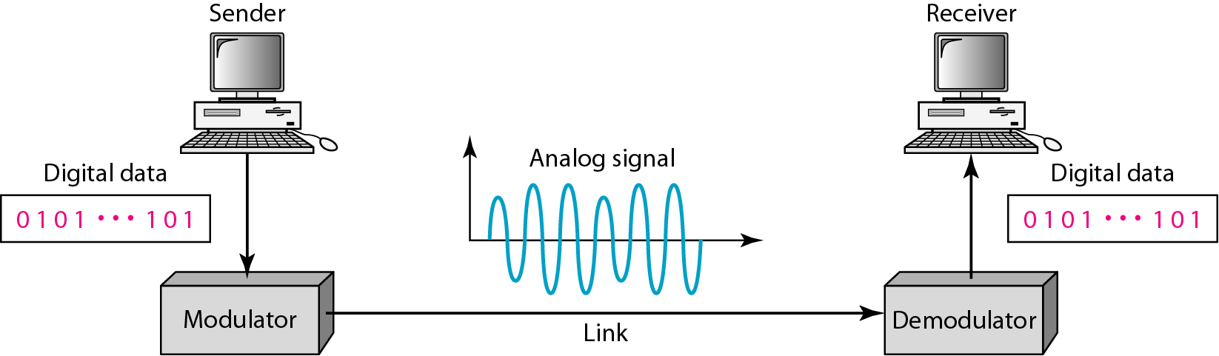
\includegraphics[width=0.9\columnwidth]{bab4/Picture1.png}
  \caption{Line coding and decoding}
  \label{fig4:1}
\end{figure}

\subsection*{Characteristics}
Before discussing different line coding schemes, we address their common characteristics.

\textbf{Signal Element Versus Data Element} Let us distinguish between a data element and a signal element. In data communications, our goal is to send data elements. A data element is the smallest entity that can represent a piece of information: this is the bit. In digital data communications, a signal element carries data elements. A signal element is the shortest unit (timewise) of a digital signal. In other words, data elements are what we need to send; signal elements are what we can send. Data elements are being carried; signal elements are the carriers.

We define a ratio r which is the number of data elements carried by each signal element. Figure 4.2 shows several situations with different values of r. In part a of the figure, one data element is carried by one signal element (r = 1). In part b of the figure, we need two signal elements (two transitions) to carry each data element (r = 1). We will see later that the extra signal element is needed to guarantee 2 synchronization. In part c ofthe figure, a signal element carries two data elements (r = 2). Finally, in part d, a group of 4 bits is being carried by a group of three signal elements (r = $\frac{4}{3}$). For every line coding scheme we discuss, we will give the value of r.

\begin{figure}[htbp]
  \centering
  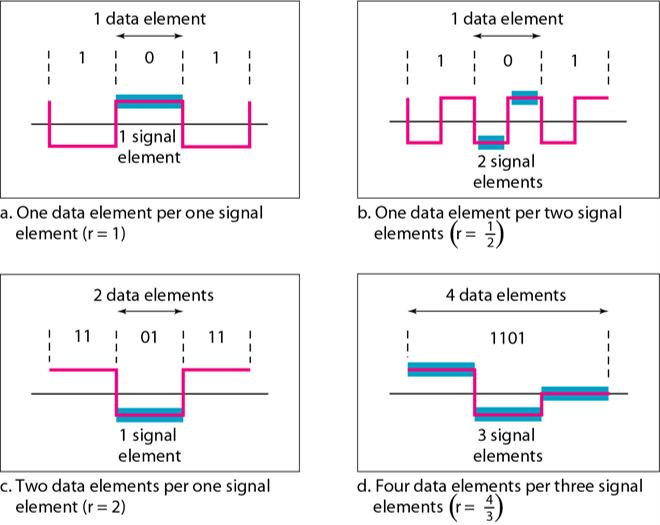
\includegraphics[width=0.9\columnwidth]{bab4/Picture2.png}
  \caption{Signal element versus data element}
  \label{fig4:2}
\end{figure}

An analogy may help here. Suppose each data element IS a person who needs to be carried from one place to another. We can think of a signal element as a vehicle that can carry people. When r = 1, it means each person is driving a vehicle. When r > 1, it means more than one person is travelling in a vehicle (a carpool, for example). We can also have the case where one person is driving a car and a trailer (r = $\frac{1}{2}$).

Data Rate Versus Signal Rate The data rate defines the number of data elements (bits) sent in Is. The unit is bits per second (bps). The signal rate is the number of signal elements sent in Is. The unit is the baud. There are several common terminologies used in the literature. The data rate is sometimes called the bit rate; the signal rate is sometimes called the pulse rate, the modulation rate, or the baud rate.

One goal in data communications is to increase the data rate while decreasing the signal rate. Increasing the data rate increases the speed of transmission; decreasing the signal rate decreases the bandwidth requirement. In our vehicle-people analogy, we need to carry more people in fewer vehicles to prevent traffic jams. We have a limited bandwidth in our transportation system.

We now need to consider the relationship between data rate and signal rate (bit rate and baud rate). This relationship, of course, depends on the value of r. It also depends on the data pattern. If we have a data pattern of all 1s or all Os, the signal rate may be different from a data pattern of alternating Os and Is. To derive a formula for the relationship, we need to define three cases: the worst, best, and average. The worst case is when we need the maximum signal rate; the best case is when we need the minimum. In data communications, we are usually interested in the average case. We can formulate the relationship between data rate and signal rate as

\begin{equation}
  S = c \times N \times \frac{1}{r} \textnormal{ baud}
\end{equation}

\noindent where N is the data rate (bps); c is the case factor, which varies for each case; S is the number of signal elements; and r is the previously defined factor.

\vspace{12pt}

\begin{example}
  A signal is carrying data in which one data element is encoded as one signal element (r = 1). If the bit rate is 100 kbps, what is the average value of the baud rate if c is between 0 and l?
\end{example}

\begin{solution}
  We assume that the average value of c is $\frac{1}{2}$. The baud rate is then

  \begin{equation*}
    S = c \times N \times \frac{1}{r} = \frac{1}{2} \times 100000 \times 1 = 50000 \textnormal{ baud} = 50 \textnormal{ kbaud}
  \end{equation*}
\end{solution}

Bandwidth We discussed in Chapter 3 that a digital signal that carries infonnation is nonperiodic. We also showed that the bandwidth of a nonperiodic signal is continuous with an infinite range. However, most digital signals we encounter in real life have a bandwidth with finite values. In other words, the bandwidth is theoretically infinite, but many of the components have such a small amplitude that they can be ignored. The effective bandwidth is finite. From now on, when we talk about the bandwidth of a digital signal, we need to remember that we are talking about this effective bandwidth. Although the actual bandwidth ofa digitalsignal is infinite, the effective bandwidth isfinite.

We can say that the baud rate, not the bit rate, determines the required bandwidth for a digital signal. If we use the transpOltation analogy, the number of vehicles affects the traffic, not the number of people being carried. More changes in the signal mean injecting more frequencies into the signal. (Recall that frequency means change and change means frequency.) The bandwidth reflects the range of frequencies we need. There is a relationship between the baud rate (signal rate) and the bandwidth. Bandwidth is a complex idea. When we talk about the bandwidth, we normally define a range of frequencies. We need to know where this range is located as well as the values of the lowest and the highest frequencies. In addition, the amplitude (if not the phase) of each component is an impOltant issue. In other words, we need more information about the bandwidth than just its value; we need a diagram of the bandwidth. We will show the bandwidth for most schemes we discuss in the chapter. For the moment, we can say that the bandwidth (range of frequencies) is proportional to the signal rate (baud rate). The minimum bandwidth can be given as

\begin{equation}
  B_{min} = c \times N \times \frac{1}{r}
\end{equation}

We can solve for the maximum data rate if the bandwidth of the channel is given.

\begin{equation}
  N_{max} = \frac{1}{c} \times B \times r
\end{equation}

\vspace{12pt}

\begin{example}
  The maximum data rate of a channel is $N_{max} = 2 \times B \times log_2L$ (defined by the Nyquist formula). Does this agree with the previous formula for $N_{max}$?
\end{example}

\begin{solution}
  A signal with L levels actually can carry $\log_2L$ bits per level. If each level corresponds to one signal element and we assume the average case (c = $\frac{1}{2}$), then we have

  \begin{equation*}
    N_{max} = \frac{1}{c} \times B \times r = 2 \times B \times \log_2L
  \end{equation*}
\end{solution}

\textbf{Baseline Wandering} In decoding a digital signal, the receiver calculates a running average of the received signal power. This average is called the baseline. The incoming signal power is evaluated against this baseline to determine the value of the data element. A long string of Os or 1s can cause a drift in the baseline (baseline wandering) and make it difficult for the receiver to decode correctly. A good line coding scheme needs to prevent baseline wandering.

\textbf{DC Components} When the voltage level in a digital signal is constant for a while, the spectrum creates very low frequencies (results of Fourier analysis). These frequencies around zero, called DC (direct-current) components, present problems for a system that cannot pass low frequencies or a system that uses electrical coupling (via a transformer). For example, a telephone line cannot pass frequencies below 200 Hz. Also a long-distance link may use one or more transformers to isolate different parts of the line electrically. For these systems, we need a scheme with no DC component.

\textbf{Self-synchronization} To correctly interpret the signals received from the sender, the receiver's bit intervals must correspond exactly to the sender's bit intervals. If the receiver clock is faster or slower, the bit intervals are not matched and the receiver might misinterpret the signals. Figure 4.3 shows a situation in which the receiver has a shorter bit duration. The sender sends 10110001, while the receiver receives 110111000011.

\begin{figure}
  \centering
  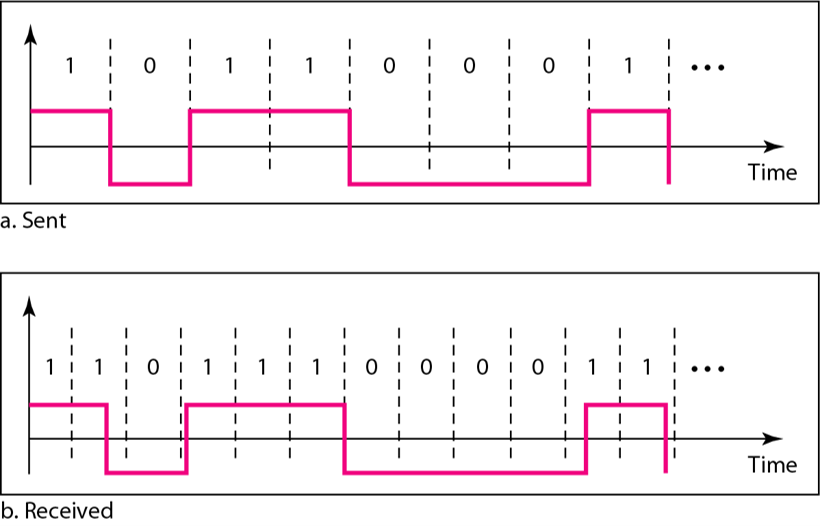
\includegraphics[width=0.9\columnwidth]{bab4/Picture3.png}
  \caption{Effect of lack of synchronization}
  \label{fig4:3}
\end{figure}

A self-synchronizing digital signal includes timing information in the data being transmitted. This can be achieved if there are transitions in the signal that alert the receiver to the beginning, middle, or end of the pulse. If the receiver's clock is out of synchronization, these points can reset the clock.

\vspace{12pt}

\begin{example}
  In a digital transmission, the receiver clock is 0.1 percent faster than the sender clock. How many extra bits per second does the receiver receive if the data rate is 1 kbps? How many if the data rate is 1 Mbps?
\end{example}

\begin{solution}
  At 1 kbps, the receiver receives 1001 bps instead of 1000 bps.

  1000 bits sent $\quad \rightarrow \quad$ 1001 bits received $\quad \rightarrow \quad$ 1 extra bps

  \noindent At 1 Mbps, the receiver receives 1,001,000 bps instead of 1,000,000 bps

  1,000,000 bits sent $\quad \rightarrow \quad$ 1,001,000 bits received $\quad \rightarrow \quad$ 1000 extra bps
\end{solution}

\vspace{6pt}

\textbf{Built-in Error Detection} It is desirable to have a built-in error-detecting capability in the generated code to detect some of or all the errors that occurred during transmission. Some encoding schemes that we will discuss have this capability to some extent

\textbf{Immunity to Noise and Interference} Another desirable code characteristic is a code I that is immune to noise and other interferences. Some encoding schemes that we will discuss have this capability. 

\textbf{Complexity} A complex scheme is more costly to implement than a simple one. For example, a scheme that uses four signal levels is more difficult to interpret than one that uses only two levels.

\subsection{Line Coding Schemes}
We can roughly divide line coding schemes into five broad categories, as shown in Figure 4.4. There are several schemes in each category. We need to be familiar with all schemes discussed in this section to understand the rest of the book. This section can be used as a reference for schemes encountered later.

\begin{figure}
  \centering
  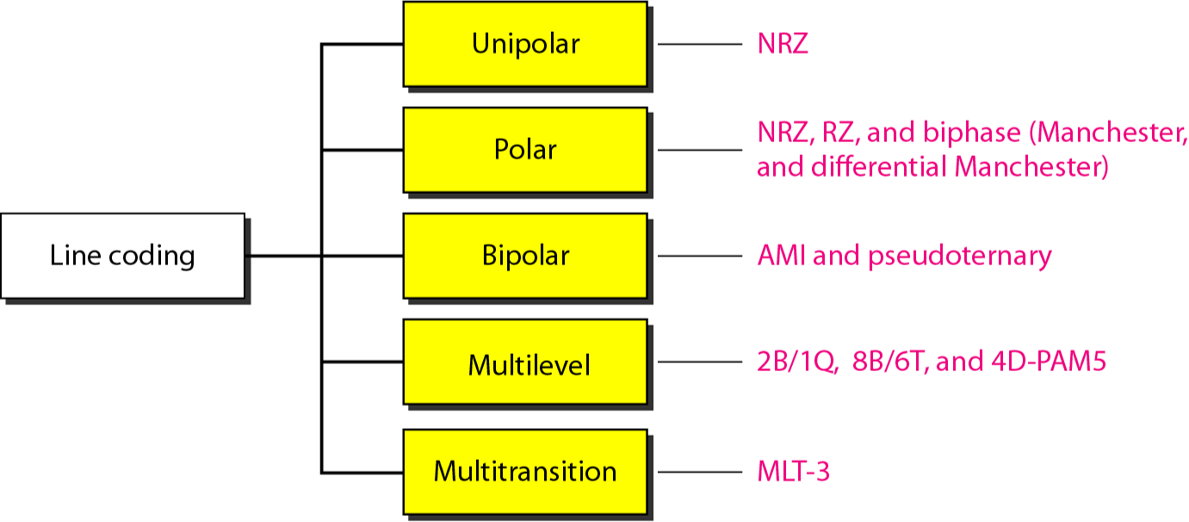
\includegraphics[width=0.9\columnwidth]{bab4/Picture4.png}
  \caption{Line coding schemes}
  \label{fig4:4}
\end{figure}

\subsection*{Unipolar Scheme}
\textbf{NRZ (Non-Return-to-Zero)} Traditionally, a unipolar scheme was designed as a non-return-to-zero (NRZ) scheme in which the positive voltage defines bit I and the zero voltage defines bit O. It is called NRZ because the signal does not return to zero at the middle of the bit. Figure 4.5 show a unipolar NRZ scheme.

\begin{figure}
  \centering
  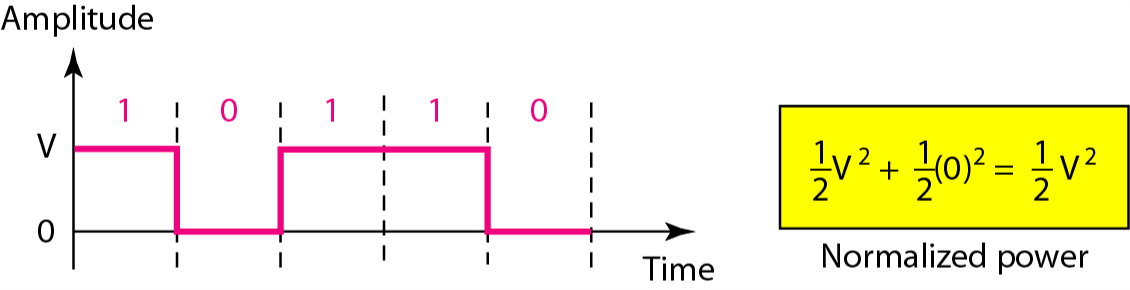
\includegraphics[width=0.9\columnwidth]{bab4/Picture5.png}
  \caption{Unipolar NRZ scheme}
  \label{fig4:5}
\end{figure}

Compared with its polar counterpart (see the next section), this scheme is very costly. As we will see shortly, the normalized power (power needed to send 1 bit per unit line resistance) is double that for polar NRZ. For this reason, this scheme is normally not used in data communications today. In a unipolar scheme, all the signal levels are on one side of the time axis, either above or below.

\subsection*{Polar Schemes}
In polar schemes, the voltages are on the both sides of the time axis. For example, the voltage level for 0 can be positive and the voltage level for I can be negative.

Non-Return-to-Zero (NRZ) In polar NRZ encoding, we use two levels of voltage amplitude. We can have two versions of polar NRZ: NRZ-Land NRZ-I, as shown in Figure 4.6. The figure also shows the value of r, the average baud rate, and the bandwidth. In the first variation, NRZ-L (NRZ-Level), the level of the voltage determines the value of the bit. In the second variation, NRZ-I (NRZ-Invert), the change or lack of change in the level of the voltage determines the value of the bit. If there is no change, the bit is 0; if there is a change, the bit is 1.

\begin{figure}
  \centering
  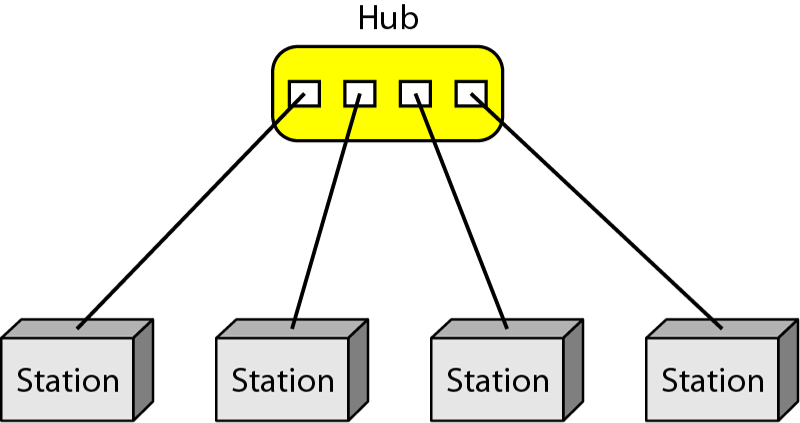
\includegraphics[width=0.9\columnwidth]{bab4/Picture6.png}
  \caption{Polar NRZ-L and NRZ-I schemes}
  \label{fig4:6}
\end{figure}

In NRZ-L the level of the voltage determines the value of the bit. In NRZ-I the inversion or the lack of inversion determines the value of the bit. Let us compare these two schemes based on the criteria we previously defined. Although baseline wandering is a problem for both variations, it is twice as severe in NRZ-L. If there is a long sequence of Os or Is in NRZ-L, the average signal power becomes skewed. The receiver might have difficulty discerning the bit value. In NRZ-I this problem occurs only for a long sequence of as. If somehow we can eliminate the long sequence of as, we can avoid baseline wandering. We will see shortly how this can be done.

The synchronization problem (sender and receiver clocks are not synchronized) also exists in both schemes. Again, this problem is more serious in NRZ-L than in NRZ-I. While a long sequence of as can cause a problem in both schemes, a long sequence of 1s affects only NRZ-L. Another problem with NRZ-L occurs when there is a sudden change of polarity in the system. For example, if twisted-pair cable is the medium, a change in the polarity of the wire results in all as interpreted as Is and all Is interpreted as as. NRZ-I does not have this problem. Both schemes have an average signal rate of
\begin{equation*}
  N/2 \textnormal{ Baud}
\end{equation*}

Let us discuss the bandwidth. Figure 4.6 also shows the normalized bandwidth for both variations. The vertical axis shows the power density (the power for each I Hz of bandwidth); the horizontal axis shows the frequency. The bandwidth reveals a very serious problem for this type of encoding. The value of the power density is velY high around frequencies close to zero. This means that there are DC components that carry a high level of energy. As a matter of fact, most of the energy is concentrated in frequencies between a and NIl. This means that although the average of the signal rate is N12, the energy is not distributed evenly between the two halves. NRZ-L and NRZ-J both have a DC component problem.

\vspace{12pt}

\begin{example}
  A system is using NRZ-I to transfer 10-Mbps data. What are the average signal rate and minimum bandwidth?
\end{example}

\begin{solution}
  The average signal rate is S =NI2 =500 kbaud. The minimum bandwidth for this average baud rate is Bnlin = S = 500 kHz.
\end{solution}

\textbf{Return to Zero (RZ)} The main problem with NRZ encoding occurs when the sender and receiver clocks are not synchronized. The receiver does not know when one bit has ended and the next bit is starting. One solution is the return-to-zero (RZ) scheme, which uses three values: positive, negative, and zero. In RZ, the signal changes not between bits but during the bit. In Figure 4.7 we see that the signal goes to 0 in the middle of each bit. It remains there until the beginning of the next bit. The main disadvantage of RZ encoding is that it requires two signal changes to encode a bit and therefore occupies greater bandwidth. The same problem we mentioned, a sudden change of polarity resulting in all as interpreted as 1s and all 1s interpreted as as, still exist here, but there is no DC component problem. Another problem is the complexity: RZ uses three levels of voltage, which is more complex to create and discern. As a result of all these deficiencies, the scheme is not used today. Instead, it has been replaced by the better-performing Manchester and differential Manchester schemes (discussed next).

\begin{figure}
  \centering
  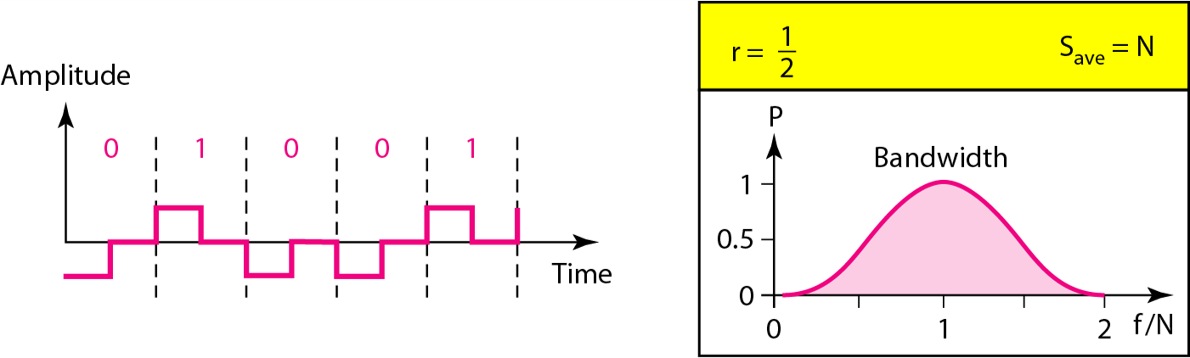
\includegraphics[width=0.9\columnwidth]{bab4/Picture7.png}
  \caption{Polar RZ scheme}
  \label{fig4:7}
\end{figure}

\textbf{Biphase: Manchester and Differential Manchester} The idea of RZ (transition at the middle of the bit) and the idea of NRZ-L are combined into the Manchester scheme. In Manchester encoding, the duration of the bit is divided into two halves. The voltage remains at one level during the first half and moves to the other level in the second half. The transition at the middle of the bit provides synchronization. Differential Manchester, on the other hand, combines the ideas of RZ and NRZ-I. There is always a transition at the middle of the bit, but the bit values are determined at the beginning of the bit. Ifthe next bit is 0, there is a transition; if the next bit is 1, there is none. Figure 4.8 shows both Manchester and differential Manchester encoding. In Manchester and differential Manchester encoding, the transition at the middle of the bit is used for synchronization.

The Manchester scheme overcomes several problems associated with NRZ-L, and differential Manchester overcomes several problems associated with NRZ-I. First, there is no baseline wandering. There is no DC component because each bit has a positive and negative voltage contribution. The only drawback is the signal rate. The signal rate for Manchester and differential Manchester is double that for NRZ. The reason is that there is always one transition at the middle of the bit and maybe one transition at the end of each bit. Figure 4.8 shows both Manchester and differential Manchester encoding schemes. Note that Manchester and differential Manchester schemes are also called biphase schemes. The minimum bandwidth ofManchester and differential Manchester is 2 times that of NRZ.

\begin{figure}[htbp]
  \centering
  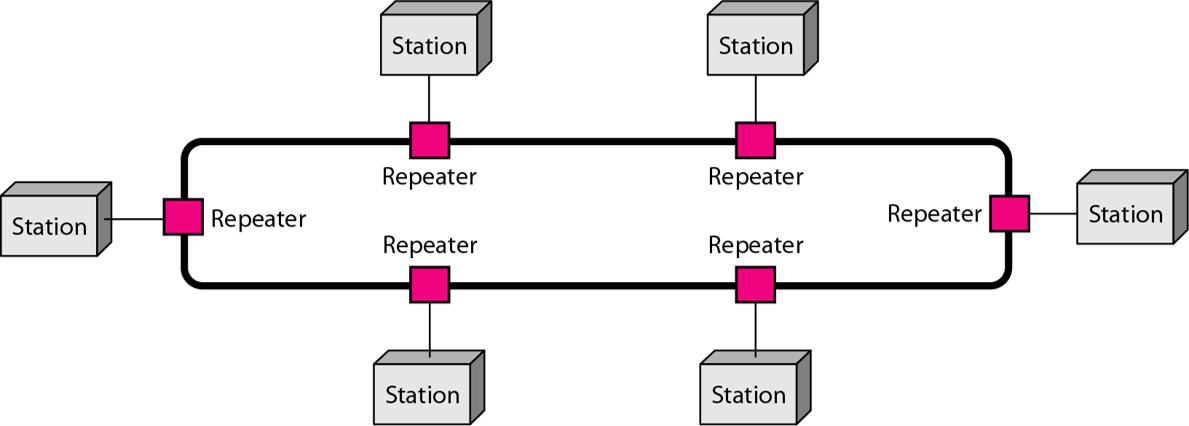
\includegraphics[width=0.9\columnwidth]{bab4/Picture8.png}
  \caption{Polar biphase schemes}
  \label{fig4:8}
\end{figure}

\subsection*{Bipolar Schemes}
In bipolar encoding (sometimes called multilevel binary), there are three voltage levels: positive, negative, and zero. The voltage level for one data element is at zero, while the voltage level for the other element alternates between positive and negative. In bipolar encoding, we use three levels: positive, zero, and negative.

\textbf{AMI and Pseudoternary} Figure 4.9 shows two variations of bipolar encoding: AMI and pseudoternary. A common bipolar encoding scheme is called bipolar alternate mark inversion (AMI). In the term alternate mark inversion, the word mark comes from telegraphy and means 1. So AMI means alternate I inversion. A neutral zero voltage represents binary O. Binary Is are represented by alternating positive and negative voltages. A variation of AMI encoding is called pseudoternary in which the 1 bit is encoded as a zero voltage and the 0 bit is encoded as alternating positive and negative voltages.

\begin{figure}
  \centering
  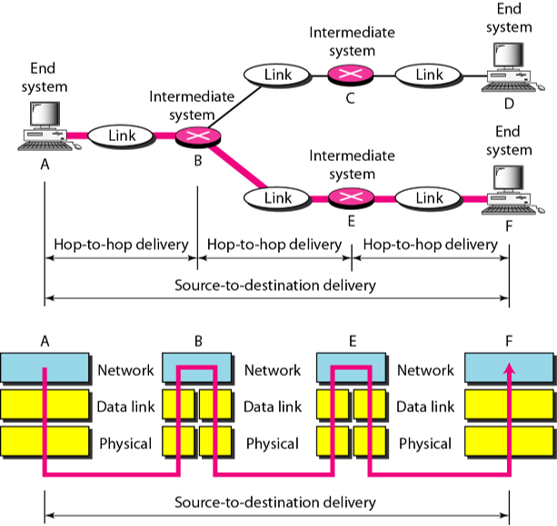
\includegraphics[width=0.9\columnwidth]{bab4/Picture9.png}
  \caption{Bipolar schemes: AMI and pseudoternary}
  \label{fig4:9}
\end{figure}

The bipolar scheme was developed as an alternative to NRZ. The bipolar scheme has the same signal rate as NRZ, but there is no DC component. The NRZ scheme has most of its energy concentrated near zero frequency, which makes it unsuitable for transmission over channels with poor performance around this frequency. The concentration of the energy in bipolar encoding is around frequency N12. Figure 4.9 shows the typical energy concentration for a bipolar scheme.

One may ask why we do not have DC component in bipolar encoding. We can answer this question by using the Fourier transform, but we can also think about it intuitively. If we have a long sequence of 1s, the voltage level alternates between positive and negative; it is not constant. Therefore, there is no DC component. For a long sequence of Os, the voltage remains constant, but its amplitude is zero, which is the same as having no DC component. In other words, a sequence that creates a constant zero voltage does not have a DC component.

AMI is commonly used for long-distance communication, but it has a synchronization problem when a long sequence of Os is present in the data. Later in the chapter, we will see how a scrambling technique can solve this problem.

\subsection*{Multilevel Schemes}
The desire to increase the data speed or decrease the required bandwidth has resulted in the creation of many schemes. The goal is to increase the number of bits per baud by encoding a pattern of m data elements into a pattern of n signal elements. We only have two types of data elements (Os and Is), which means that a group of m data elements can produce a combination of 2m data patterns. We can have different types of signal elements by allowing different signal levels. If we have L different levels, then we can produce Ln combinations of signal patterns. If 2m =Ln, then each data pattern is encoded into one signal pattern. If 2m < Ln, data patterns occupy only a subset of signal patterns. The subset can be carefully designed to prevent baseline wandering, to provide synchronization, and to detect errors that occurred during data transmission. Data encoding is not possible if 2m > Ln because some of the data patterns cannot be encoded.

The code designers have classified these types of coding as mBnL, where m is the length of the binary pattern, B means binary data, n is the length of the signal pattern, and L is the number of levels in the signaling. A letter is often used in place of L: B (binary) for L =2, T (ternary) for L =3, and Q (quaternary) for L =4. Note that the first two letters define the data pattern, and the second two define the signal pattern. In mBnL schemes, a pattern ofm data elements is encoded as a pattern ofn signal elements in which 2m ::::; Ln.

2BIQ The first mBnL scheme we discuss, two binary, one quaternary (2BIQ), uses data patterns of size 2 and encodes the 2-bit patterns as one signal element belonging to a four-level signal. In this type of encoding m =2, n =1, and L =4 (quatemary). Figure 4.10 shows an example of a 2B1Q signal.

The average signal rate of 2BlQ is S =N/4. This means that using 2BIQ, we can send data 2 times faster than by using NRZ-L. However, 2B lQ uses four different signal levels, which means the receiver has to discern four different thresholds. The reduced bandwidth comes with a price. There are no redundant signal patterns in this scheme because 22 =41 .

\begin{figure}
  \centering
  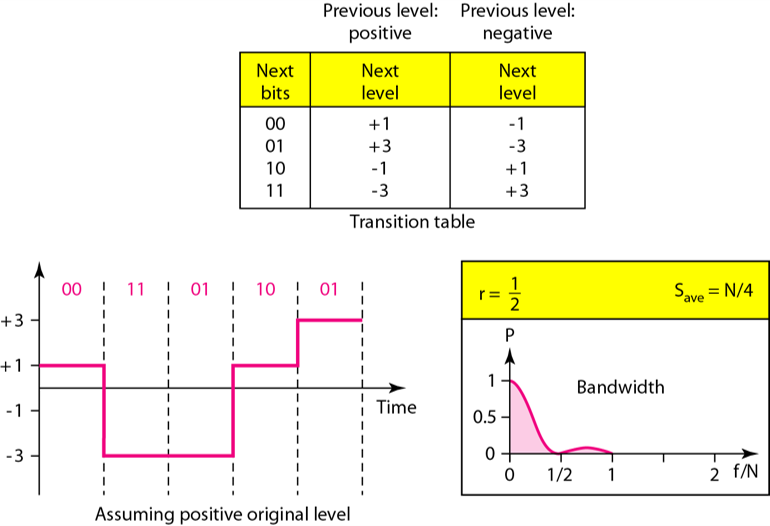
\includegraphics[width=0.9\columnwidth]{bab4/Picture10.png}
  \caption{Multilevel: 2B1Q scheme}
  \label{fig4:10}
\end{figure}

8B6T A very interesting scheme is eight binary, six ternary (8B6T). This code is used with 100BASE-4T cable, as we will see in Chapter 13. The idea is to encode a pattern of 8 bits as a pattern of 6 signal elements, where the signal has three levels (ternary). In this type of scheme, we can have 28 =256 different data patterns and 36 =478 different signal patterns. The mapping table is shown in Appendix D. There are 478 - 256 =222 redundant signal elements that provide synchronization and error detection. Part of the redundancy is also used to provide DC balance. Each signal pattern has a weight of 0 or +1 DC values. This means that there is no pattern with the weight -1. To make the whole stream Dc-balanced, the sender keeps track of the weight. If two groups of weight 1 are encountered one after another, the first one is sent as is, while the next one is totally inverted to give a weight of -1.

Figure 4.11 shows an example of three data patterns encoded as three signal patterns. The three possible signal levels are represented as -,0, and +. The first 8-bit pattern 00010001 is encoded as the signal pattern -0-0++ with weight 0; the second 8-bit pattern 010 10011 is encoded as - + - + + 0 with weight +1. The third bit pattern should be encoded as + - - + 0 + with weight +1. To create DC balance, the sender inverts the actual signal. The receiver can easily recognize that this is an inverted pattern because the weight is -1. The pattern is inverted before decoding. The average signal rate of the scheme is theoretically Save = ! X N X §; in practice the minimum bandwidth is very close to 6N18.

\begin{figure}[htbp]
  \centering
  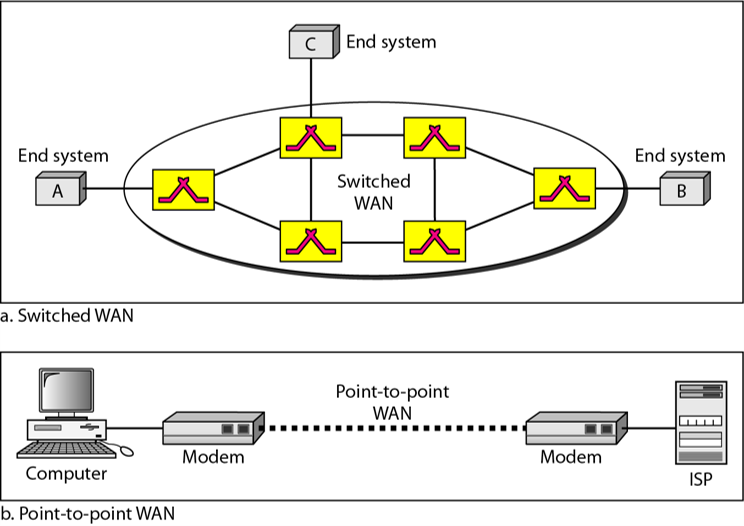
\includegraphics[width=0.9\columnwidth]{bab4/Picture11.png}
  \caption{Multilevel: 8B6T scheme}
  \label{fig4:11}
\end{figure}

4D-PAMS The last signaling scheme we discuss in this category is called fourdimensional five-level pulse amplitude modulation (4D-PAM5). The 4D means that data is sent over four wires at the same time. It uses five voltage levels, such as -2, -1, 0, 1, and 2. However, one level, level 0, is used only for forward error detection. If we assume that the code is just one-dimensional, the four levels create something similar to 8B4Q. In other words, an 8-bit word is translated to a signal element offour different levels. The worst signal rate for this imaginary one-dimensional version is N X 4/8, orN12.

The technique is designed to send data over four channels (four wires). This means the signal rate can be reduced to N18, a significant achievement. All 8 bits can be fed into a wire simultaneously and sent by using one signal element. The point here is that the four signal elements comprising one signal group are sent simultaneously in a four-dimensional setting. Figure 4.12 shows the imaginary one-dimensional and the actual four-dimensional implementation. Gigabit LANs use this technique to send 1-Gbps data over four copper cables that can handle 125 Mbaud. This scheme has a lot of redundancy in the signal pattern because 28 data patterns are matched to 44 = 256 signal patterns. The extra signal patterns can be used for other purposes such as error detection.

\begin{figure}
  \centering
  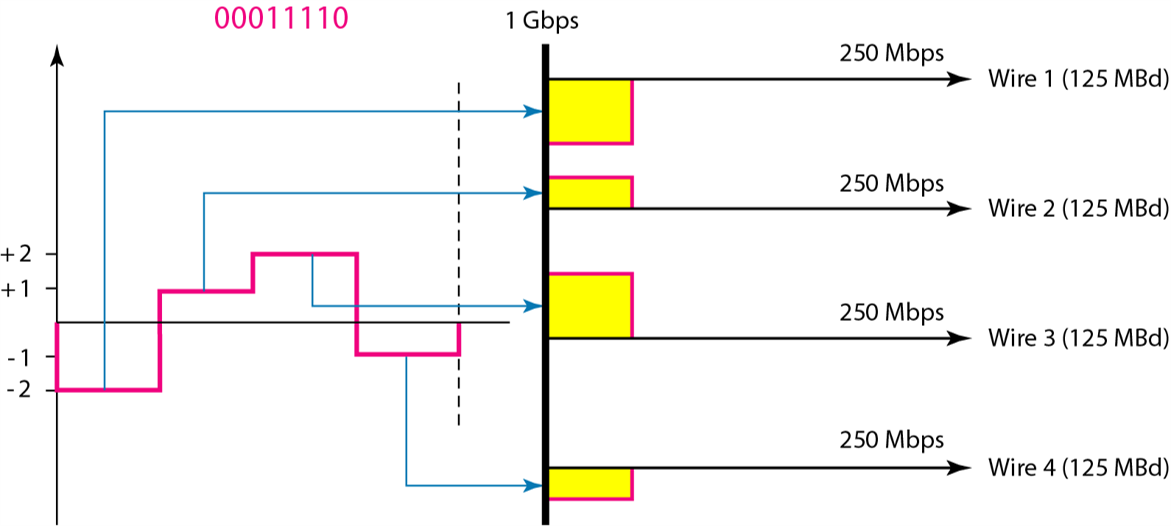
\includegraphics[width=0.9\columnwidth]{bab4/Picture12.png}
  \caption{Multilevel: 4D-PAM5 scheme}
  \label{fig4:12}
\end{figure}

\subsection*{Multiline Transmission: MLT-3}
NRZ-I and differential Manchester are classified as differential encoding but use two transition rules to encode binary data (no inversion, inversion). Ifwe have a signal with more than two levels, we can design a differential encoding scheme with more than two transition rules. MLT-3 is one of them. The multiline transmission, three level (MLT-3) scheme uses three levels (+v, 0, and - V) and three transition rules to move between the levels.
\begin{enumerate}
  \item If the next bit is 0, there is no transition.
  \item If the next bit is 1 and the current level is not 0, the next level is 0.
  \item If the next bit is 1 and the cutTent level is 0, the next level is the opposite of the last nonzero level
\end{enumerate}

The behavior of MLT-3 can best be described by the state diagram shown in Figure 4.13. The three voltage levels (-V, 0, and +V) are shown by three states (ovals). The transition from one state (level) to another is shown by the connecting lines. Figure 4.13 also shows two examples of an MLT-3 signal.

\begin{figure}
  \centering
  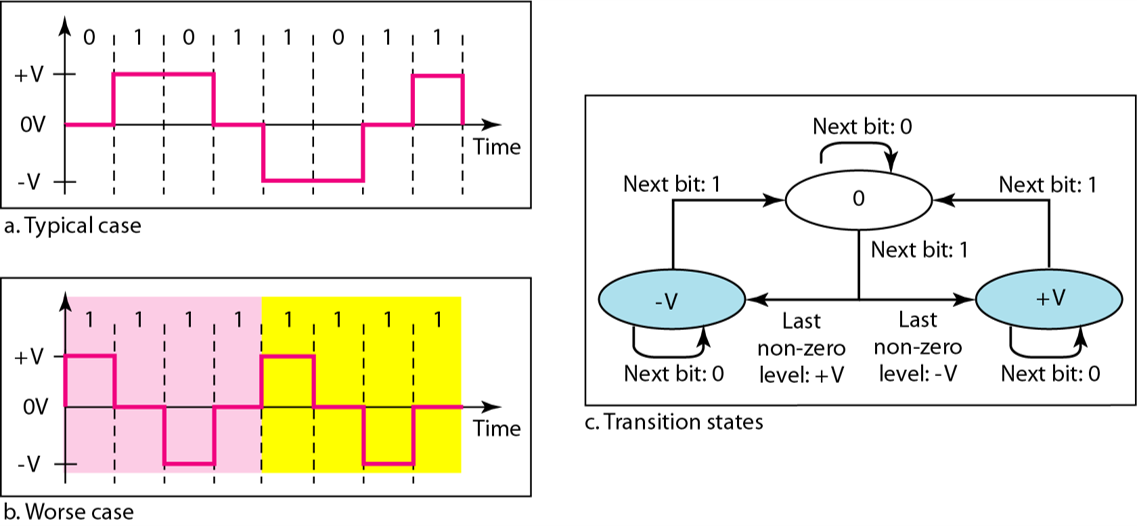
\includegraphics[width=0.9\columnwidth]{bab4/Picture13.png}
  \caption{Multitransition: MLT-3 scheme}
  \label{fig4:13}
\end{figure}

One might wonder why we need to use MLT-3, a scheme that maps one bit to one signal element. The signal rate is the same as that for NRZ-I, but with greater complexity (three levels and complex transition rules). It turns out that the shape of the signal in this scheme helps to reduce the required bandwidth. Let us look at the worst-case scenario, a sequence of Is. In this case, the signal element pattern +VO - VO is repeated every 4 bits. A nonperiodic signal has changed to a periodic signal with the period equal to 4 times the bit duration. This worst-case situation can be simulated as an analog signal with a frequency one-fourth of the bit rate. In other words, the signal rate for MLT-3 is one-fourth the bit rate. This makes MLT-3 a suitable choice when we need to send 100 Mbps on a copper wire that cannot support more than 32 MHz (frequencies above this level create electromagnetic emissions).

\subsection*{Summary ofLine Coding Schemes}
We summarize in Table 4.1 the characteristics of the different schemes discussed.

\begin{table}[htbp]
  \begin{center}
    \centering
    \caption{Ringkasan skema \textit{line coding}}
    \begin{tabular}{|l|l|c|p{6cm}|}
      \cline{1-4}
      \multirow{2}{*}{Kategori} & \multirow{2}{*}{Skema} & \multicolumn{1}{c|}{Bandwidth} & \multirow{2}{*}{\centerline{Karakteristik}} \\
      & & \multicolumn{1}{c|}{(rata-rata)} & \\
      \cline{1-4}
      Unipolar & NRZ & B=N/2 & Mahal, tidak ada \textit{self-synchronization} jika panjang 0s atau 1s, DC \\
      \cline{1-4}
      \multirow{3}{*}{Unipolar} & NRZ-L & B=N/2 & Tidak ada \textit{self-synchronization} jika 0s panjang atau 1s, DC \\
      \cline{2-4}
      & NRZ-I & B=N/2 & Tidak ada \textit{self-synchronization} selama S, DC \\
      \cline{2-4}
      & Biphase & B=N & \textit{self-synchronization}, tidak ada DC, bandwidth tinggi \\
      \cline{1-4}
      Bipolar & AMI & B=N/2 & Tidak ada \textit{self-synchronization} untuk 0s lama, DC \\
      \cline{1-4}
      \multirow{3}{*}{Multilevel} & 2BIQ & B=N/4 & Tidak ada \textit{self-synchronization} untuk bit ganda yang sama panjang \\
      \cline{2-4}
      & 8B6T & B=3N/4 & \textit{self-synchronization}, tidak ada DC \\
      \cline{2-4}
      & 4D-PAM5 & B=N/8 & \textit{self-synchronization}, tidak ada DC \\
      \cline{1-4}
      Multiline & MLT-3 & B=N/3 & Tidak ada \textit{self-synchronization} untuk 0s yang lama \\
      \cline{1-4}
    \end{tabular}
  \end{center}\vspace*{6px}
\end{table}\vspace*{8px}

\subsection{Block Coding}
We need redundancy to ensure synchronization and to provide some kind of inherent error detecting. Block coding can give us this redundancy and improve the performance of line coding. In general, block coding changes a block of m bits into a block of n bits, where n is larger than m. Block coding is referred to as an mB/nB encoding technique. Block coding is normally referred to as mBlnB coding; it replaces each m~bit group with an n~bit group.

The slash in block encoding (for example, 4B/5B) distinguishes block encoding from multilevel encoding (for example, 8B6T), which is written without a slash. Block coding normally involves three steps: division, substitution, and combination. In the division step, a sequence of bits is divided into groups of m bits. For example, in 4B/5B encoding, the original bit sequence is divided into 4-bit groups. The heart of block coding is the substitution step. In this step, we substitute an m-bit group for an n-bit group. For example, in 4B/5B encoding we substitute a 4-bit code for a 5-bit group. Finally, the n-bit groups are combined together to form a stream. The new stream has more bits than the original bits. Figure 4.14 shows the procedure.

\begin{figure}
  \centering
  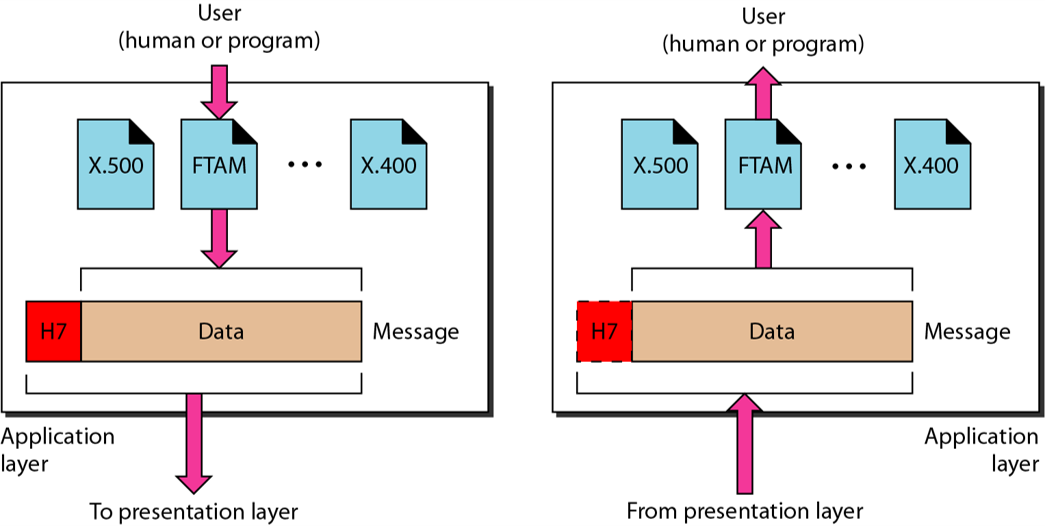
\includegraphics[width=0.9\columnwidth]{bab4/Picture14.png}
  \caption{Block coding concept}
  \label{fig4:14}
\end{figure}

\subsection*{4B/5B} 
The four binary/five binary (4B/5B) coding scheme was designed to be used in combination with NRZ-I. Recall that NRZ-I has a good signal rate, one-half that of the biphase, but it has a synchronization problem. A long sequence of as can make the receiver clock lose synchronization. One solution is to change the bit stream, prior to encoding with NRZ-I, so that it does not have a long stream of as. The 4B/5B scheme achieves this goal. The block-coded stream does not have more that three consecutive as, as we will see later. At the receiver, the NRZ-I encoded digital signal is first decoded into a stream of bits and then decoded to remove the redundancy. Figure 4.15 shows the idea.

In 4B/5B, the 5-bit output that replaces the 4-bit input has no more than one leading zero (left bit) and no more than two trailing zeros (right bits). So when different groups are combined to make a new sequence, there are never more than three consecutive as. (Note that NRZ-I has no problem with sequences of Is.) Table 4.2 shows the corresponding pairs used in 4B/5B encoding. Note that the first two columns pair a 4-bit group with a 5-bit group. A group of 4 bits can have only 16 different combinations while a group of 5 bits can have 32 different combinations. This means that there are 16 groups that are not used for 4B/5B encoding. Some of these unused groups are used for control purposes; the others are not used at all. The latter provide a kind of error detection. If a 5-bit group arrives that belongs to the unused portion of the table, the receiver knows that there is an error in the transmission.

\begin{figure}
  \centering
  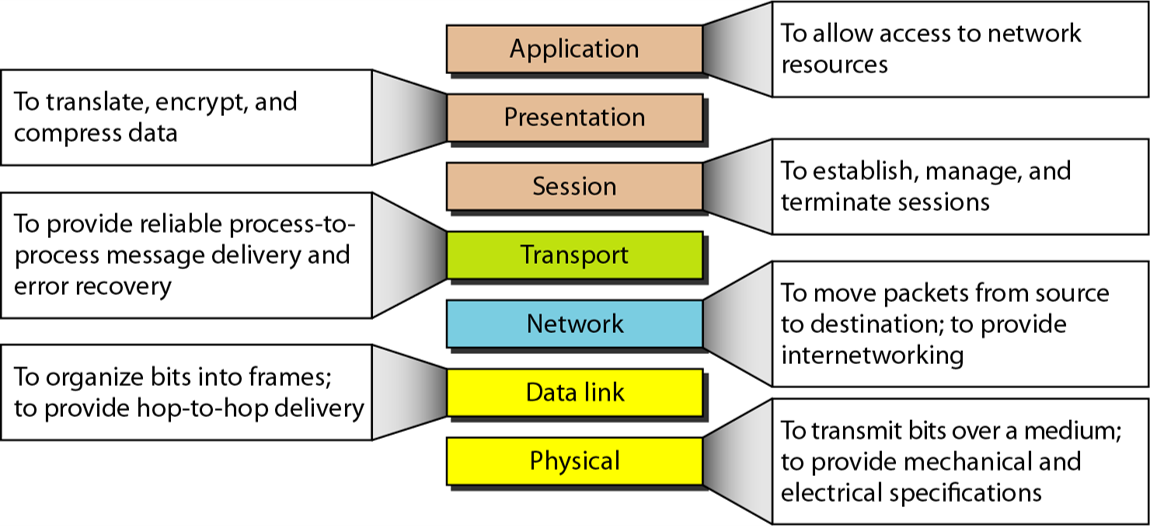
\includegraphics[width=0.9\columnwidth]{bab4/Picture15.png}
  \caption{Using block coding 4B/5B with NRZ-I line coding scheme}
  \label{fig4:15}
\end{figure}

\begin{table}
  \centering
  \caption{4B/5B mapping codes}
  \begin{tabular}{| c | c | c | c |}
    \hline
    Data Sequence & Encoded Sequence & Control sequence & encoded sequence \\
    \hline
    0000 & 11110 & Q (Quiet) & 00000 \\
    \hline  
    0001 & 01001 & I (Idle) & 11111 \\
    \hline
    0010 & 10100 & H (Halt) & 00100 \\
    \hline
    0011 & 10101 & J (Start delimeter) & 11000 \\
    \hline
    0100 & 01010 & K (Start delimeter) & 10001 \\
    \hline
    0101 & 01011 & T (End delimeter) & 01101 \\
    \hline
    0110 & 01110 & S (Set) & 11001 \\
    \hline
    0111 & 01111 & R (Reset) & 00111 \\
    \hline
    1000 & 10010 &  &  \\
    \hline
    1001 & 10011 &  &  \\
    \hline
    1010 & 10110 &  &  \\
    \hline
    1011 & 10111 &  &  \\
    \hline
    1100 & 11010 &  &  \\
    \hline
    1101 & 11011 &  &  \\
    \hline
    1110 & 11100 &  &  \\
    \hline
    1111 & 11101 &  &  \\
    \hline
  \end{tabular}
\end{table}

Figure 4.16 shows an example of substitution in 4B/5B coding. 4B/5B encoding solves the problem of synchronization and overcomes one of the deficiencies of NRZ-1. However, we need to remember that it increases the signal rate of NRZ-1. The redundant bits add 20 percent more baud. Still, the result is less than the biphase scheme which has a signal rate of 2 times that of NRZ-1. However, 4B/5B block encoding does not solve the DC component problem of NRZ-1. If a DC component is unacceptable, we need to use biphase or bipolar encoding.

\begin{figure}[htbp]
  \centering
  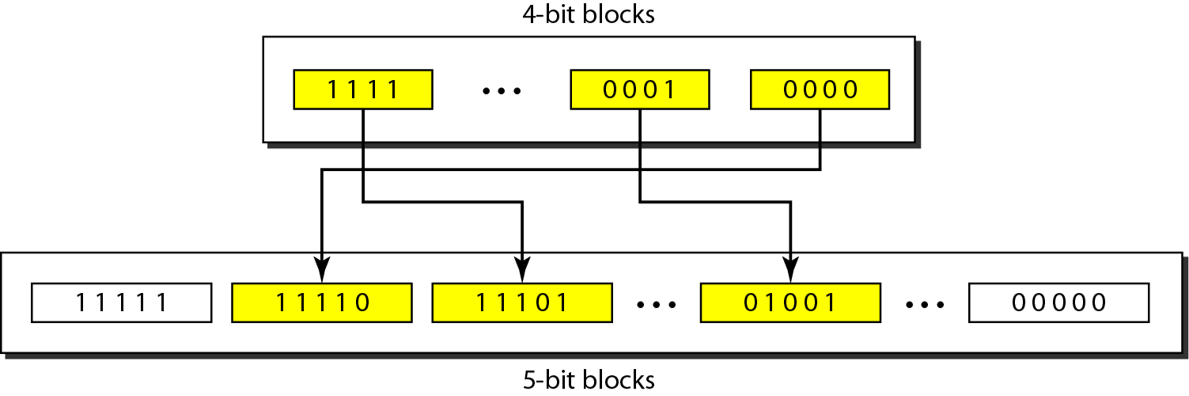
\includegraphics[width=0.9\columnwidth]{bab4/Picture16.png}
  \caption{Substitution in 48/5B block coding}
  \label{fig4:16}
\end{figure}

\vspace{12pt}

\begin{example}
  We need to send data at a 1-Mbps rate. What is the minimum required bandwidth, using a combination of 4B/5B and NRZ-I or Manchester coding?
\end{example}

\begin{solution}
  First 4B/5B block coding increases the bit rate to 1.25 Mbps. The minimum bandwidth using NRZ-I is NI2 or 625 kHz. The Manchester scheme needs a minimum bandwidth of 1 MHz. The first choice needs a lower bandwidth, but has a DC component problem; the second choice needs a higher bandwidth, but does not have a DC component problem.
\end{solution}

\subsection*{8RIlOR}
The eight binary/ten binary (SBIlOB) encoding is similar to 4B/5B encoding except that a group of 8 bits of data is now substituted by a lO-bit code. It provides greater error detection capability than 4B/5B. The 8BIlOB block coding is actually a combination of 5B/6B and 3B/4B encoding, as shown in Figure 4.17

\begin{figure}
  \centering
  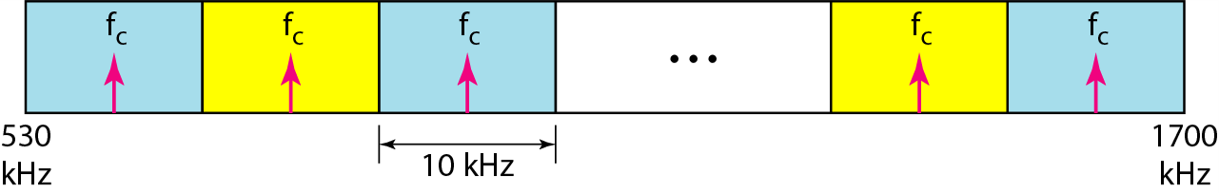
\includegraphics[width=0.9\columnwidth]{bab4/Picture17.png}
  \caption{8B/lOB block encoding}
  \label{fig4:17}
\end{figure}

The most five significant bits of a 10-bit block is fed into the 5B/6B encoder; the least 3 significant bits is fed into a 3B/4B encoder. The split is done to simplify the mapping table. To prevent a long run of consecutive Os or Is, the code uses a disparity controller which keeps track of excess Os over Is (or Is over Os). If the bits in the current block create a disparity that contributes to the previous disparity (either direction), then each bit in the code is complemented (a 0 is changed to a 1 and a 1 is changed to a 0). The coding has 210 - 28 =768 redundant groups that can be used for disparity checking and error detection. In general, the technique is superior to 4B/5B because of better built-in error-checking capability and better synchronization.

\subsection{Scrambling}
Biphase schemes that are suitable for dedicated links between stations in a LAN are not suitable for long-distance communication because of their wide bandwidth requirement. The combination of block coding and NRZ line coding is not suitable for long-distance encoding either, because of the DC component. Bipolar AMI encoding, on the other hand, has a narrow bandwidth and does not create a DC component. However, a long sequence of Os upsets the synchronization. Ifwe can find a way to avoid a long sequence of Os in the original stream, we can use bipolar AMI for long distances. We are looking for a technique that does not increase the number of bits and does provide synchronization. We are looking for a solution that substitutes long zero-level pulses with a combination of other levels to provide synchronization. One solution is called scrambling. We modify part of the AMI rule to include scrambling, as shown in Figure 4.18. Note that scrambling, as opposed to block coding, is done at the same time as encoding. The system needs to insert the required pulses based on the defined scrambling rules. Two common scrambling techniques are B8ZS and HDB3.

\begin{figure}
  \centering
  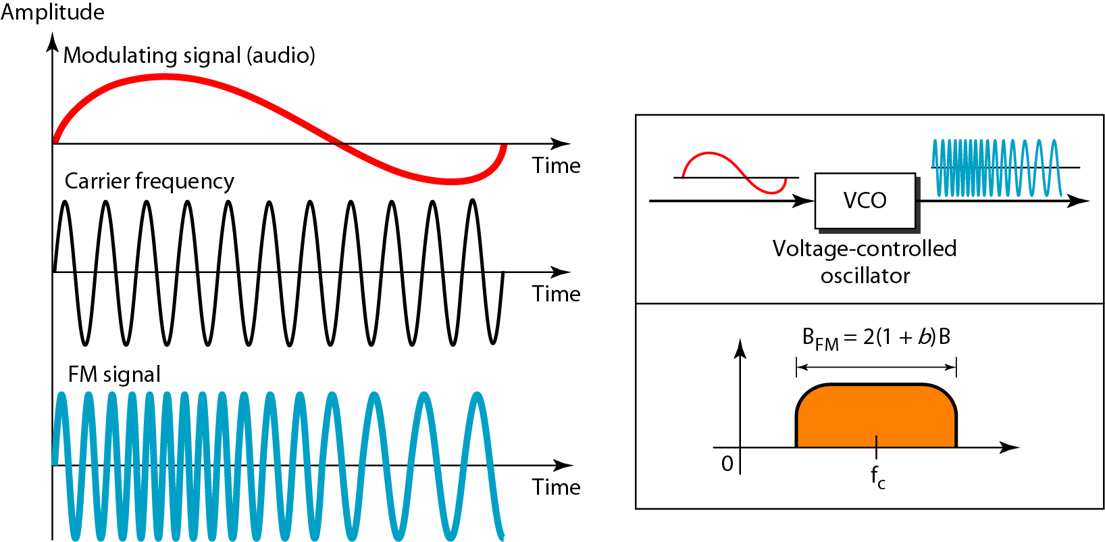
\includegraphics[width=0.9\columnwidth]{bab4/Picture18.png}
  \caption{AMI used with scrambling}
  \label{fig4:18}
\end{figure}

\subsection*{R8ZS}
Bipolar with S-zero substitution (BSZS) is commonly used in North America. In this technique, eight consecutive zero-level voltages are replaced by the sequence OOOVBOVB. The V in the sequence denotes violation; this is a nonzero voltage that breaks an AMI rule of encoding (opposite polarity from the previous). The B in the sequence denotes bipolm; which means a nonzero level voltage in accordance with the AMI rule. There are two cases, as shown in Figure 4.19.

\begin{figure}
  \centering
  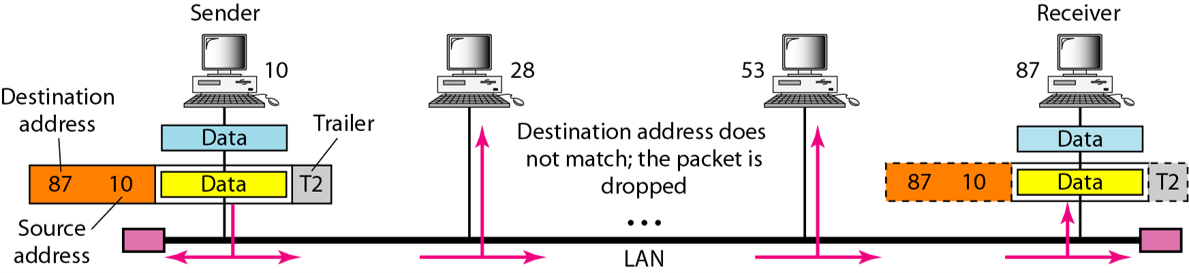
\includegraphics[width=0.9\columnwidth]{bab4/Picture19.png}
  \caption{Two cases ofB8ZS scrambling technique}
  \label{fig4:19}
\end{figure}

Note that the scrambling in this case does not change the bit rate. Also, the technique balances the positive and negative voltage levels (two positives and two negatives), which means that the DC balance is maintained. Note that the substitution may change the polarity of a 1 because, after the substitution, AMI needs to follow its rules. B8ZS substitutes eight consecutive zeros with OOOVBOVB. One more point is worth mentioning. The letter V (violation) or B (bipolar) here is relative. The V means the same polarity as the polarity of the previous nonzero pulse; B means the polarity opposite to the polarity of the previous nonzero pulse.

\subsection*{HDB3}
High-density bipolar 3-zero (HDB3) is commonly used outside of North America. In this technique, which is more conservative than B8ZS, four consecutive zero-level voltages are replaced with a sequence of OOOV or BOO\: The reason for two different substitutions is to maintain the even number of nonzero pulses after each substitution. The two rules can be stated as follows:
\begin{enumerate}
  \item If the number of nonzero pulses after the last substitution is odd, the substitution pattern will be OOOV, which makes the total number of nonzero pulses even.
  \item If the number of nonzero pulses after the last substitution is even, the substitution pattern will be BOOV, which makes the total number of nonzero pulses even.
\end{enumerate}

Figure 4.20 shows an example. There are several points we need to mention here. First, before the first substitution, the number of nonzero pulses is even, so the first substitution is BODY. After this substitution, the polarity of the 1 bit is changed because the AMI scheme, after each substitution, must follow its own rule. After this bit, we need another substitution, which is OOOV because we have only one nonzero pulse (odd) after the last substitution. The third substitution is BOOV because there are no nonzero pulses after the second substitution (even). HDB3 substitutes four consecutive zeros with OOOV or BOOV depending on the number of nonzero pulses after the last substitution.

\begin{figure}
  \centering
  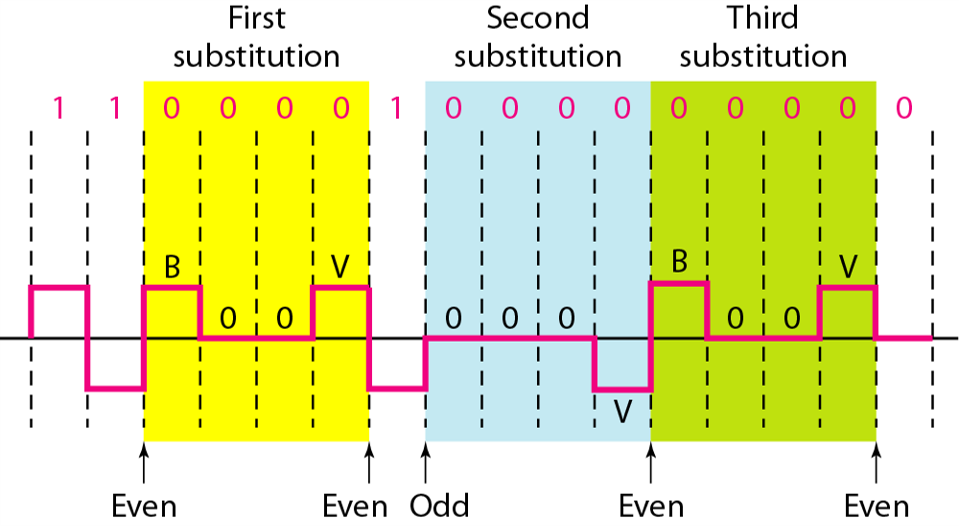
\includegraphics[width=0.9\columnwidth]{bab4/Picture20.png}
  \caption{Different situations in HDB3 scrambling technique}
  \label{fig4:20}
\end{figure}

\section{Konversi Analog to Digital}
The techniques described in Section 4.1 convert digital data to digital signals. Sometimes, however, we have an analog signal such as one created by a microphone or camera. We have seen in Chapter 3 that a digital signal is superior to an analog signal. The tendency today is to change an analog signal to digital data. In this section we describe two techniques, pulse code modulation and delta modulation. After the digital data are created (digitization), we can use one of the techniques described in Section 4.1 to convert the digital data to a digital signal.

\subsection{Pulse Code Modulation (PCM)}
The most common technique to change an analog signal to digital data (digitization) is called pulse code modulation (PCM). A PCM encoder has three processes, as shown in Figure 4.21.
\begin{enumerate}
  \item The analog signal is sampled.
  \item The sampled signal is quantized.
  \item The quantized values are encoded as streams of bits.
\end{enumerate}

\begin{figure}
  \centering
  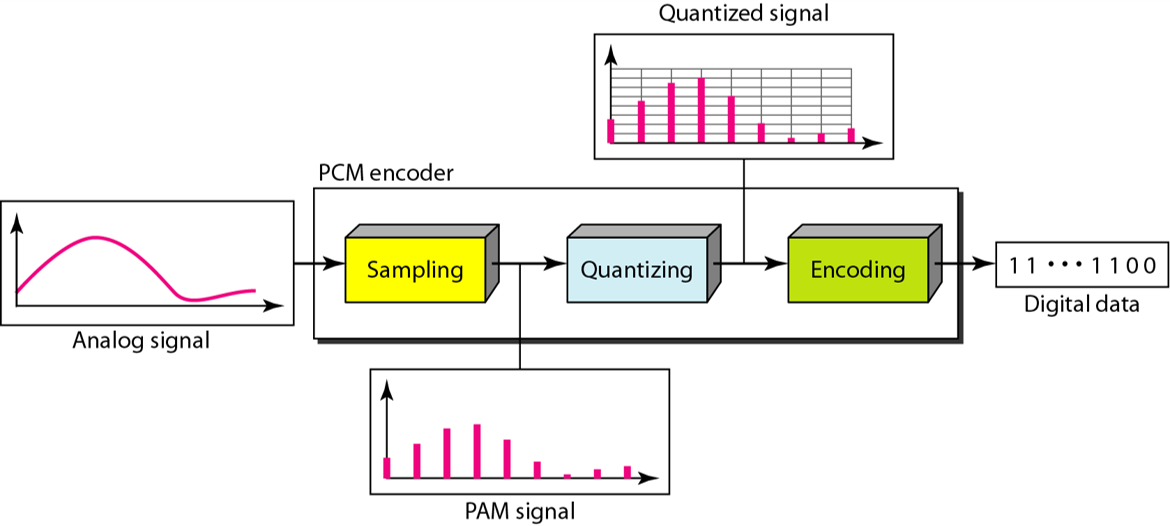
\includegraphics[width=0.9\columnwidth]{bab4/Picture21.png}
  \caption{Components ofPCM encoder}
  \label{fig4:21}
\end{figure}

\subsection*{Sampling}
The first step in PCM is sampling. The analog signal is sampled every Ts s, where Ts is the sample interval or period. The inverse of the sampling interval is called the sampling rate or sampling frequency and denoted by is, where is = IITs ' There are three sampling methods-ideal, natural, and flat-top-as shown in Figure 4.22.

In ideal sampling, pulses from the analog signal are sampled. This is an ideal sampling method and cannot be easily implemented. In natural sampling, a high-speed switch is turned on for only the small period of time when the sampling occurs. The result is a sequence of samples that retains the shape of the analog signal. The most common sampling method, called sample and hold, however, creates flat-top samples by using a circuit. The sampling process is sometimes referred to as pulse amplitude modulation (PAM). We need to remember, however, that the result is still an analog signal with nonintegral values.

Sampling Rate One important consideration is the sampling rate or frequency. What are the restrictions on Ts? This question was elegantly answered by Nyquist. According to the Nyquist theorem, to reproduce the original analog signal, one necessary condition is that the sampling rate be at least twice the highest frequency in the original signal.

\begin{figure}
  \centering
  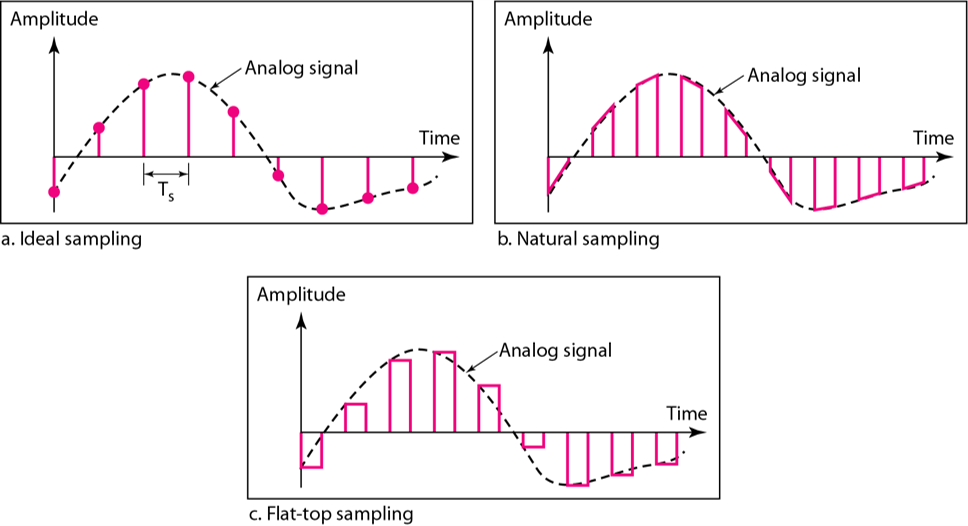
\includegraphics[width=0.9\columnwidth]{bab4/Picture22.png}
  \caption{Three different sampling methodsfor PCM}
  \label{fig4:22}
\end{figure}

According to the Nyquist theorem, the sampling rate must be at least 2 times the highest frequency contained in the signal. We need to elaborate on the theorem at this point. First, we can sample a signal only if the signal is band-limited. In other words, a signal with an infinite bandwidth cannot be sampled. Second, the sampling rate must be at least 2 times the highest frequency, not the bandwidth. If the analog signal is low-pass, the bandwidth and the highest frequency are the same value. If the analog signal is bandpass, the bandwidth value is lower than the value of the maximum frequency. Figure 4.23 shows the value of the sampling rate for two types of signals.

\begin{figure}
  \centering
  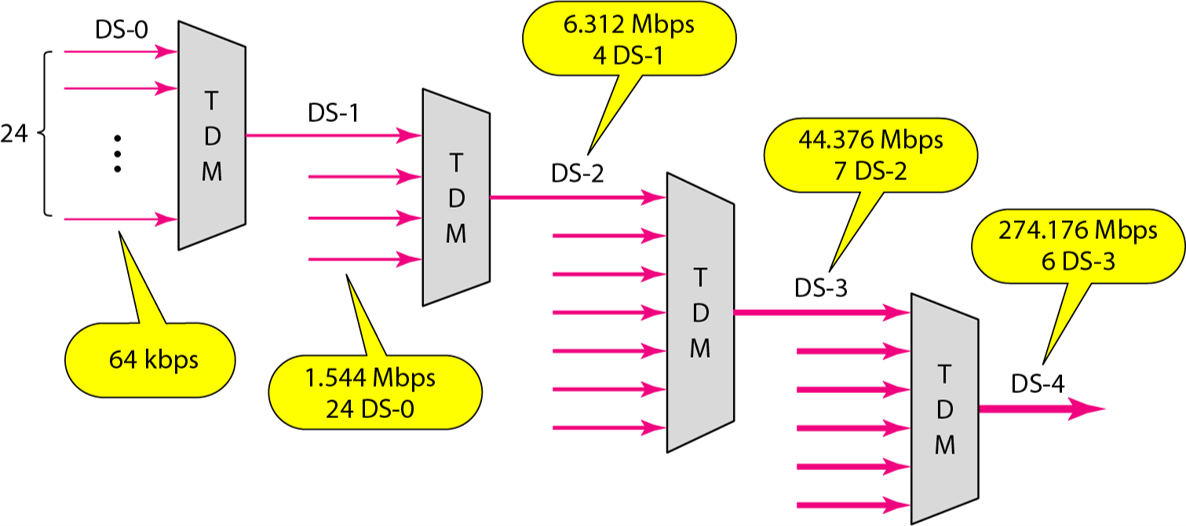
\includegraphics[width=0.9\columnwidth]{bab4/Picture23.png}
  \caption{Nyquist sampling rate for low-pass and bandpass signals}
  \label{fig4:23}
\end{figure}

\begin{example}
  For an intuitive example of the Nyquist theorem, let us sample a simple sine wave at three sampling rates: fs = 4f (2 times the Nyquist rate )'/s = 2f (Nyquist rate), and fs =f (one-half the Nyquist rate). Figure 4.24 shows the sampling and the subsequent recovery of the signal.
\end{example}

\begin{figure}
  \centering
  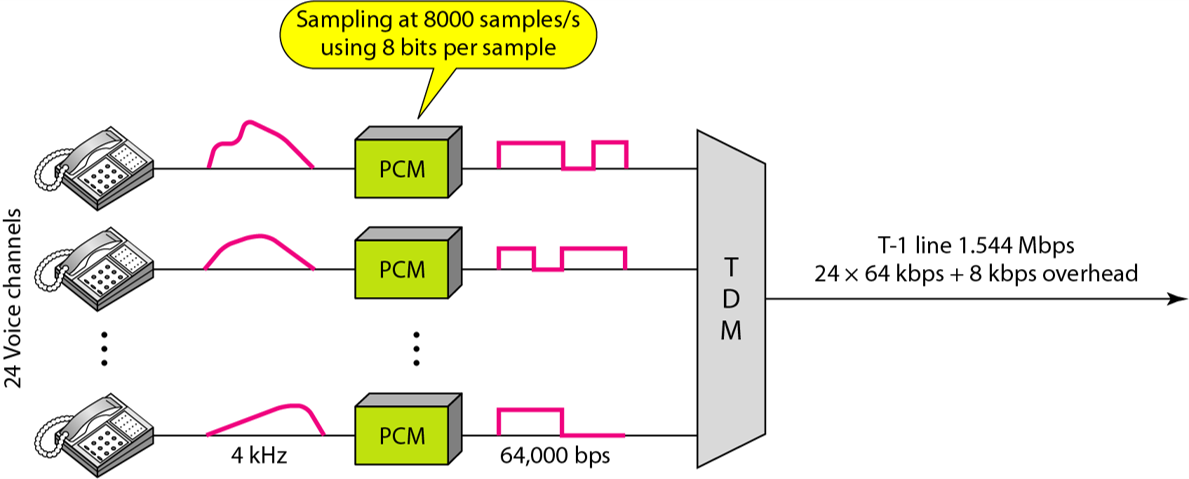
\includegraphics[width=0.9\columnwidth]{bab4/Picture24.png}
  \caption{Recovery ofa sampled sine wave for different sampling rates}
  \label{fig4:24}
\end{figure}

It can be seen that sampling at the Nyquist rate can create a good approximation of the original sine wave (part a). Oversampling in part b can also create the same approximation, but it is redundant and unnecessary. Sampling below the Nyquist rate (part c) does not produce a signal that looks like the original sine wave.

\begin{example}
  As an interesting example, let us see what happens if we sample a periodic event such as the revolution of a hand of a clock. The second hand of a clock has a period of 60 s. According to the Nyquist theorem, we need to sample the hand (take and send a picture) every 30 s (Ts = Tor fs = 2f). In Figure 4.25a, the sample points, in order, are 12, 6, 12, 6, 12, and 6. The receiver of the samples cannot tell if the clock is moving forward or backward. In part b, we sample at double the Nyquist rate (every 15 s). The sample points, in order, are 12,3,6, 9, and 12. The clock is moving forward. In part c, we sample below the Nyquist rate (Ts = Torfs =~f). The sample points, in order, are 12, 9,6,3, and 12. Although the clock is moving forward, the receiver thinks that the clock is moving backward
\end{example}

\begin{figure}[htbp]
  \centering
  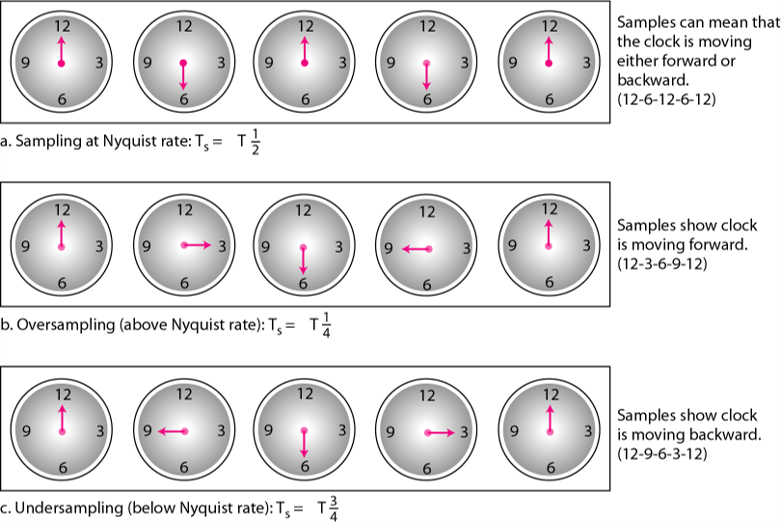
\includegraphics[width=0.9\columnwidth]{bab4/Picture25.png}
  \caption{Sampling ofa clock with only one hand}
  \label{fig4:25}
\end{figure}

\vspace{12pt}

\begin{example}
  An example related to Example 4.7 is the seemingly backward rotation of the wheels of a forwardmoving car in a movie. This can be explained by undersampling. A movie is filmed at 24 frames per second. If a wheel is rotating more than 12 times per second, the undersampling creates the impression of a backward rotation
\end{example}

\vspace{12pt}

\begin{example}
  Telephone companies digitize voice by assuming a maximum frequency of 4000 Hz. The sampling rate therefore is 8000 samples per second.
\end{example}

\vspace{12pt}

\begin{example}
  A complex low-pass signal has a bandwidth of 200 kHz. What is the minimum sampling rate for this signal?
\end{example}

\begin{solution}
  The bandwidth of a low-pass signal is between 0 andj, where f is the maximum frequency in the signal. Therefore, we can sample this signal at 2 times the highest frequency (200 kHz). The sampling rate is therefore 400,000 samples per second.
\end{solution}

\vspace{12pt}

\begin{example}
  A complex bandpass signal has a bandwidth of 200 kHz. What is the minimum sampling rate for this signal?
\end{example}

\begin{solution}
  We cannot find the minimum sampling rate in this case because we do not know where the bandwidth starts or ends. We do not know the maximum frequency in the sign
\end{solution}

\subsection*{Quantization}
The result of sampling is a series of pulses with amplitude values between the maximum and minimum amplitudes of the signal. The set of amplitudes can be infinite with nonintegral values between the two limits. These values cannot be used in the encoding process. The following are the steps in quantization:
\begin{enumerate}
  \item We assume that the original analog signal has instantaneous amplitudes between Vmin and Vmax'
  \item We divide the range into L zones, each of height $\Delta$ (delta).
  \begin{equation*}
    \Delta = \frac{V_{max} - V_{min}}{L}
  \end{equation*}
  \item We assign quantized values of 0 to L - 1 to the midpoint of each zone.
  \item We approximate the value of the sample amplitude to the quantized values.
\end{enumerate}

As a simple example, assume that we have a sampled signal and the sample amplitudes are between -20 and +20 V. We decide to have eight levels (L = 8). This means that =5 V. Figure 4.26 shows this example.

\begin{figure}[htbp]
  \centering
  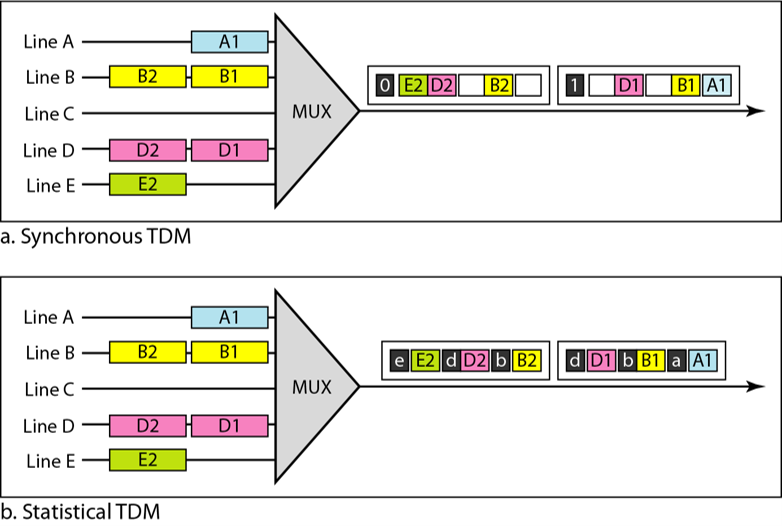
\includegraphics[width=0.9\columnwidth]{bab4/Picture26.png}
  \caption{Quantization and encoding ofa sampled signal}
  \label{fig4:26}
\end{figure}

We have shown only nine samples using ideal sampling (for simplicity). The value at the top of each sample in the graph shows the actual amplitude. In the chart, the first row is the normalized value for each sample (actual amplitude/.:1). The quantization process selects the quantization value from the middle of each zone. This means that the normalized quantized values (second row) are different from the normalized amplitudes. The difference is called the normalized error (third row). The fourth row is the quantization code for each sample based on the quantization levels at the left of the graph. The encoded words (fifth row) are the final products of the conversion.

Quantization Levels In the previous example, we showed eight quantization levels. The choice of L, the number of levels, depends on the range of the amplitudes of the analog signal and how accurately we need to recover the signal. If the amplitude of a signal fluctuates between two values only, we need only two levels; if the signal, like voice, has many amplitude values, we need more quantization levels. In audio digitizing, L is normally chosen to be 256; in video it is normally thousands. Choosing lower values of L increases the quantization error if there is a lot of fluctuation in the signal.

Quantization Error One important issue is the error created in the quantization process. (Later, we will see how this affects high-speed modems.) Quantization is an approximation process. The input values to the quantizer are the real values; the output values are the approximated values. The output values are chosen to be the middle value in the zone. If the input value is also at the middle of the zone, there is no quantization error; otherwise, there is an error. In the previous example, the normalized amplitude of the third sample is 3.24, but the normalized quantized value is 3.50. This means that there is an error of +0.26. The value of the error for any sample is less than .:112. In other words, we have -.:112 -::;; error -::;; .:112.

The quantization error changes the signal-to-noise ratio of the signal, which in turn reduces the upper limit capacity according to Shannon. It can be proven that the contribution of the quantization error to the SNRdB of the signal depends on the number of quantization levels L, or the bits per sample nb' as shown in the following formula:

\begin{equation}
  SNR_{dB} =6.02\textnormal{nb} + 1.76 \textnormal{ dB}
\end{equation}

\vspace{12pt}

\begin{example}
  What is the SNRdB in the example of Figure 4.26?
\end{example}

\begin{solution}
  We can use the formula to find the quantization. We have eight levels and 3 bits per sample, so SNRdB =6.02(3) + 1.76 = 19.82 dB. Increasing the number of levels increases the SNR.
\end{solution}

\vspace{12pt}

\begin{example}
  A telephone subscriber line must have an SN~B above 40. What is the minimum number of bits per sample?
\end{example}

\begin{solution}
  We can calculate the number of bits as
  \begin{equation*}
    SN~:::: 6.02nb + 1.76:::: 40 ..... n:::: 6.35
  \end{equation*}
  \noindent Telephone companies usually assign 7 or 8 bits per sample.
\end{solution}

Uniform Versus Nonuniform Quantization For many applications, the distribution of the instantaneous amplitudes in the analog signal is not uniform. Changes in amplitude often occur more frequently in the lower amplitudes than in the higher ones. For these types of applications it is better to use nonuniform zones. In other words, the height of is not fixed; it is greater near the lower amplitudes and less near the higher amplitudes. Nonuniform quantization can also be achieved by using a process called companding and expanding. The signal is companded at the sender before conversion; it is expanded at the receiver after conversion. Companding means reducing the instantaneous voltage amplitude for large values; expanding is the opposite process. Companding gives greater weight to strong signals and less weight to weak ones. It has been proved that nonuniform quantization effectively reduces the SNRdB of quantization.

\subsection*{Encoding}
The last step in PCM is encoding. After each sample is quantized and the number of bits per sample is decided, each sample can be changed to an llb-bit code word. In Figure 4.26 the encoded words are shown in the last row. A quantization code of 2 is encoded as 010; 5 is encoded as 101; and so on. Note that the number of bits for each sample is determined from the number of quantization levels. If the number of quantization levels is L, the number of bits is llb =log2 L. In our example L is 8 and llb is therefore 3. The bit rate can be found from the formula

\begin{equation}
  Bit rate :::: sampling rate x number of bits per sample::::is x nb
\end{equation}

\begin{example}
  We want to digitize the human voice. What is the bit rate, assuming 8 bits per sample?
\end{example}

\begin{solution}
  The human voice normally contains frequencies from 0 to 4000 Hz. So the sampling rate and bit rate are calculated as follows:
\end{solution}

\begin{equation*}
  Sampling rate :::: 4000 x 2 :::: 8000 samples/s 
\end{equation*}

\begin{equation*}
  Bit rate == 8000 x 8 :::: 64,000 bps == 64 kbps
\end{equation*}

\subsection*{Original Signal Recovery}
The recovery of the original signal requires the PCM decoder. The decoder first uses circuitry to convert the code words into a pulse that holds the amplitude until the next pulse. After the staircase signal is completed, it is passed through a low-pass filter to smooth the staircase signal into an analog signal. The filter has the same cutoff frequency as the original signal at the sender. If the signal has been sampled at (or greater than) the Nyquist sampling rate and if there are enough quantization levels, the original signal will be recreated. Note that the maximum and minimum values of the original signal can be achieved by using amplification. Figure 4.27 shows the simplified process.

\begin{figure}
  \centering
  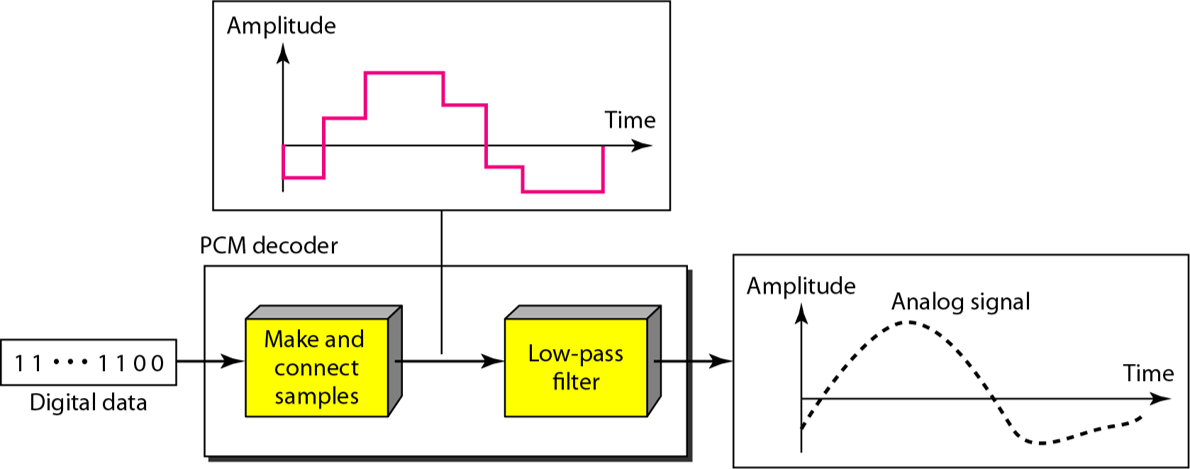
\includegraphics[width=0.9\columnwidth]{bab4/Picture27.png}
  \caption{Components ofa PCM decoder}
  \label{fig4:27}
\end{figure}

\subsection*{PCM Bandwidth}
Suppose we are given the bandwidth of a low-pass analog signal. If we then digitize the signal, what is the new minimum bandwidth of the channel that can pass this digitized signal? We have said that the minimum bandwidth of a line-encoded signal is Bmin =ex N x (lIr). We substitute the value ofN in this formula:

\begin{equation}
  Bmin =c x N x - 111
\end{equation}

\noindent When lIr = I (for a NRZ or bipolar signal) and c = (12) (the average situation), the minimum bandwidth is

\begin{equation}
  B_{min} = n_b \times B_{analog}
\end{equation}

\noindent This means the minimum bandwidth of the digital signal is nb times greater than the bandwidth of the analog signal. This is the price we pay for digitization.

\vspace{12pt}

\begin{example}
  We have a low-pass analog signal of 4 kHz. If we send the analog signal, we need a channel with a minimum bandwidth of 4 kHz. If we digitize the signal and send 8 bits per sample, we need a channel with a minimum bandwidth of 8 X 4 kHz =32 kHz.
\end{example}

\subsection*{Maximum Data Rate of a Channel}
In Chapter 3, we discussed the Nyquist theorem which gives the data rate of a channel as Nmax =2 x B x log2 L. We can deduce this rate from the Nyquist sampling theorem by using the following arguments.
\begin{enumerate}
  \item We assume that the available channel is low-pass with bandwidth B.
  \item We assume that the digital signal we want to send has L levels, where each level is a signal element. This means r = 1/10g2 L.
  \item We first pass the digital signal through a low-pass filter to cut off the frequencies above B Hz.
  \item We treat the resulting signal as an analog signal and sample it at 2 x B samples per second and quantize it using L levels. Additional quantization levels are useless because the signal originally had L levels
  \item The resulting bit rate is N =fs x nb =2 x B x log2 L. This is the maximum bandwidth; if the case factor c increases, the data rate is reduced
  \begin{equation}
    Nmax ::::: 2 x B x logzL bps
  \end{equation}
\end{enumerate}

\subsection*{Minimum Required Bandwidth}
The previous argument can give us the minimum bandwidth if the data rate and the number of signal levels are fixed. We can say
\begin{equation}
  B . = N Hz
\end{equation}

\subsection{Delta Modulation (DM)}
PCM is a very complex technique. Other techniques have been developed to reduce the complexity of PCM. The simplest is delta modulation. PCM finds the value of the signal amplitude for each sample; DM finds the change from the previous sample. Figure 4.28 shows the process. Note that there are no code words here; bits are sent one after another

\begin{figure}
  \centering
  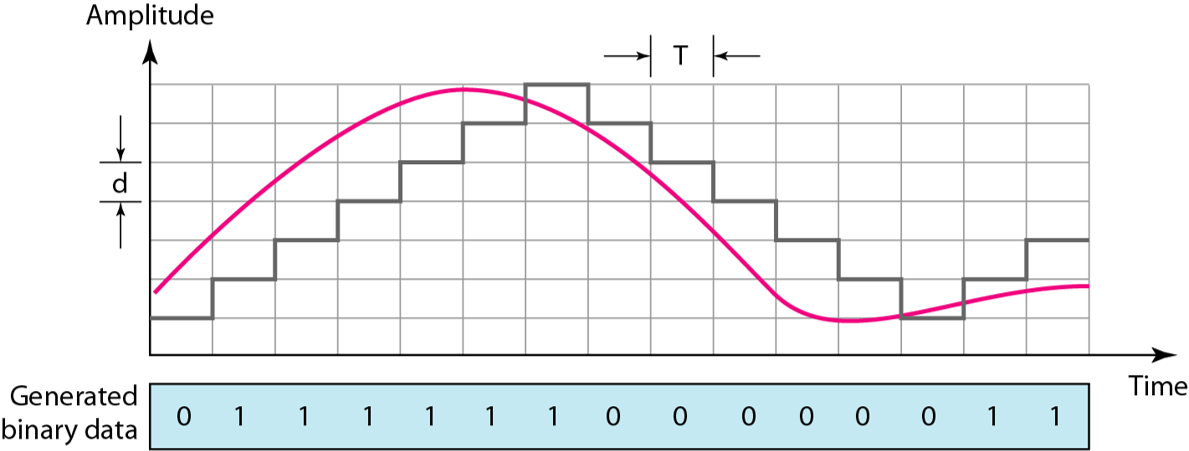
\includegraphics[width=0.9\columnwidth]{bab4/Picture28.png}
  \caption{The process ofdelta modulation}
  \label{fig4:28}
\end{figure}

\subsection*{Modulator}
The modulator is used at the sender site to create a stream of bits from an analog signal. The process records the small positive or negative changes, called delta O. Ifthe delta is positive, the process records a I; if it is negative, the process records a O. However, the process needs a base against which the analog signal is compared. The modulator builds a second signal that resembles a staircase. Finding the change is then reduced to comparing the input signal with the gradually made staircase signal. Figure 4.29 shows a diagram of the process.

\begin{figure}
  \centering
  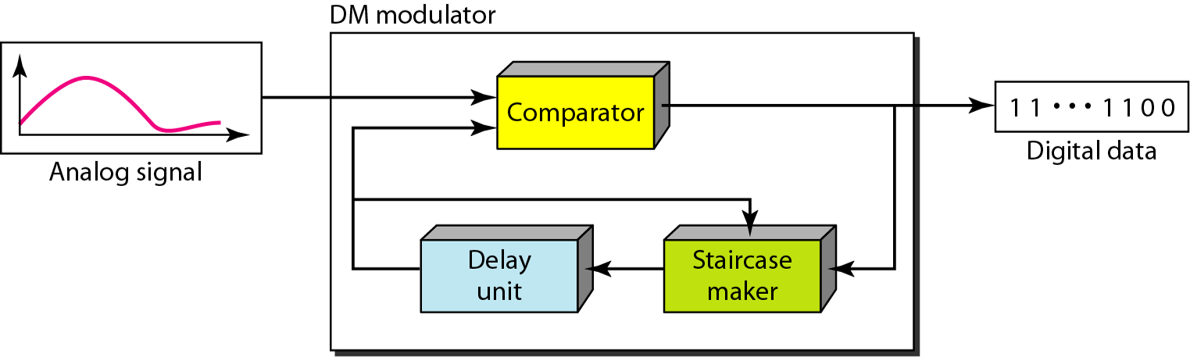
\includegraphics[width=0.9\columnwidth]{bab4/Picture29.png}
  \caption{Delta modulation components}
  \label{fig4:29}
\end{figure}

The modulator, at each sampling interval, compares the value of the analog signal with the last value of the staircase signal. Ifthe amplitude of the analog signal is larger, the next bit in the digital data is 1; otherwise, it is O. The output of the comparator, however, also makes the staircase itself. If the next bit is I, the staircase maker moves the last point of the staircase signal 0 up; it the next bit is 0, it moves it 0 down. Note that we need a delay unit to hold the staircase function for a period between two comparisons.

\subsection*{Demodulator}
The demodulator takes the digital data and, using the staircase maker and the delay unit, creates the analog signal. The created analog signal, however, needs to pass through a low-pass filter for smoothing. Figure 4.30 shows the schematic diagram.

\begin{figure}
  \centering
  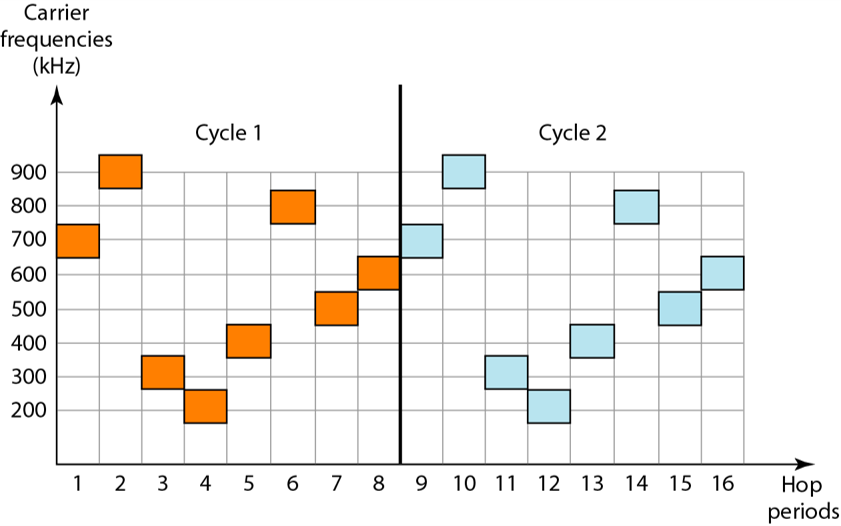
\includegraphics[width=0.9\columnwidth]{bab4/Picture30.png}
  \caption{Delta modulation components}
  \label{fig4:30}
\end{figure}

\subsection*{Adaptive DM}
A better performance can be achieved if the value of 0 is not fixed. In adaptive delta modulation, the value of 0 changes according to the amplitude of the analog signal.

\subsection*{Quantization Error}
It is obvious that DM is not perfect. Quantization error is always introduced in the process. The quantization error of DM, however, is much less than that for PCM.

\section{Mode Transmisi}
Of primary concern when we are considering the transmission of data from one device to another is the wiring, and of primary concern when we are considering the wiring is the data stream. Do we send 1 bit at a time; or do we group bits into larger groups and, if so, how?. The transmission of binary data across a link can be accomplished in either parallel or serial mode. In parallel mode, multiple bits are sent with each clock tick. In serial mode, 1 bit is sent with each clock tick. While there is only one way to send parallel data, there are three subclasses of serial transmission: asynchronous, synchronous, and isochronous (lihat gambar~\ref{fig4:31}).

\begin{figure}
  \centering
  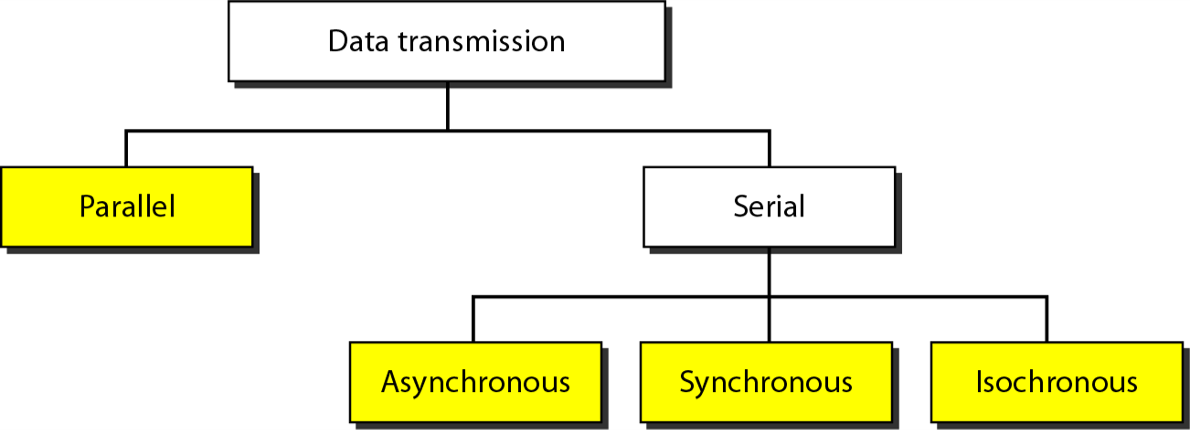
\includegraphics[width=0.9\columnwidth]{bab4/Picture31.png}
  \caption{Data transmission and modes}
  \label{fig4:31}
\end{figure}

\subsection{Parallel Transmission}
Binary data, consisting of Is and Os, may be organized into groups of n bits each. Computers produce and consume data in groups of bits much as we conceive of and use spoken language in the form of words rather than letters. By grouping, we can send data n bits at a time instead of 1. This is called parallel transmission. The mechanism for parallel transmission is a conceptually simple one: Use n wires to send n bits at one time. That way each bit has its own wire, and all n bits of one group can be transmitted with each clock tick from one device to another. Figure 4.32 shows how parallel transmission works for n =8. Typically, the eight wires are bundled in a cable with a connector at each end.

\begin{figure}
  \centering
  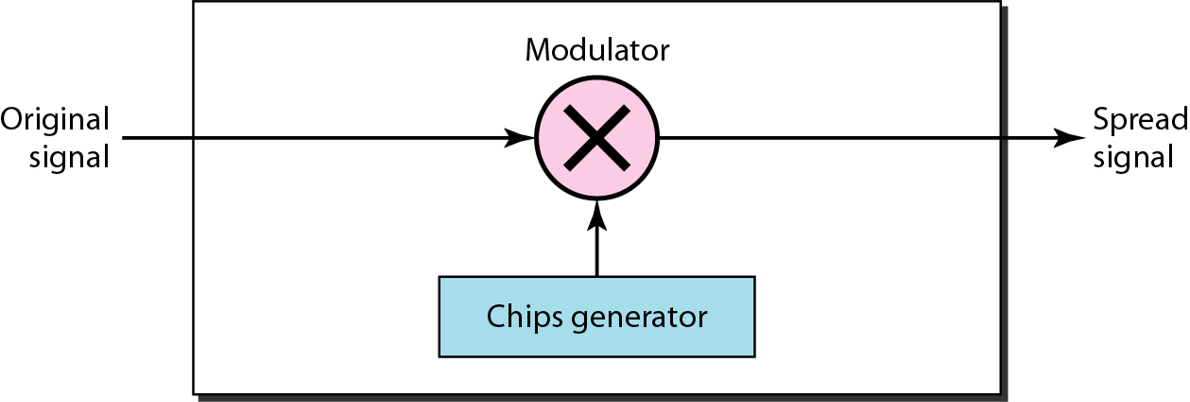
\includegraphics[width=0.9\columnwidth]{bab4/Picture32.png}
  \caption{Parallel transmission}
  \label{fig4:32}
\end{figure}

The advantage of parallel transmission is speed. All else being equal, parallel transmission can increase the transfer speed by a factor of n over serial transmission. But there is a significant disadvantage: cost. Parallel transmission requires n communication lines (wires in the example) just to transmit the data stream. Because this is expensive, parallel transmission is usually limited to short distances.

\subsection{Serial Transmission}
In serial transmission one bit follows another, so we need only one communication channel rather than n to transmit data between two communicating devices (see Figure 4.33).

\begin{figure}
  \centering
  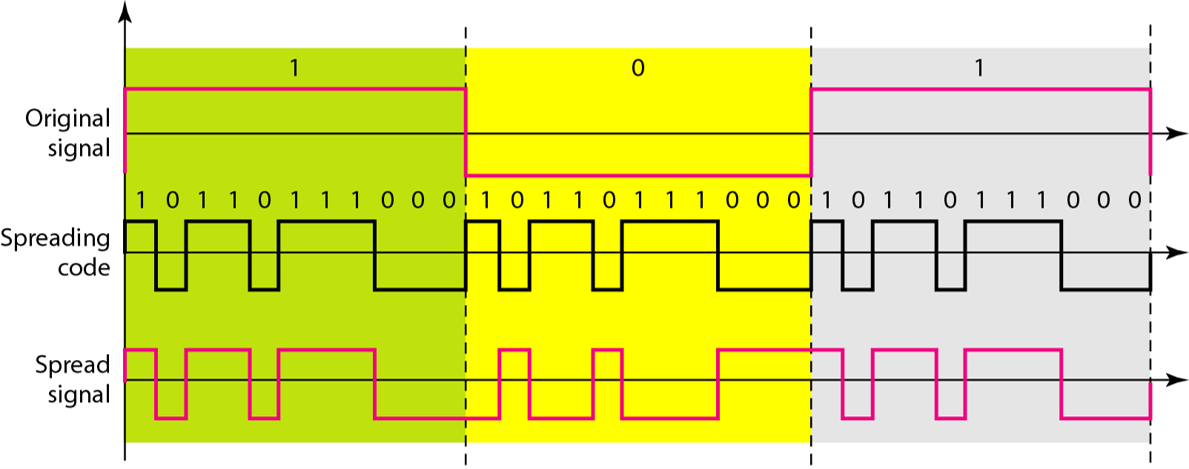
\includegraphics[width=0.9\columnwidth]{bab4/Picture33.png}
  \caption{Serial transmission}
  \label{fig4:33}
\end{figure}

The advantage of serial over parallel transmission is that with only one communication channel, serial transmission reduces the cost of transmission over parallel by roughly a factor of n. Since communication within devices is parallel, conversion devices are required at the interface between the sender and the line (parallel-to-serial) and between the line and the receiver (serial-to-parallel). Serial transmission occurs in one of three ways: asynchronous, synchronous, and isochronous.

\subsection*{Asynchronous Transmission}
Asynchronous transmission is so named because the timing of a signal is unimportant. Instead, information is received and translated by agreed upon patterns. As long as those patterns are followed, the receiving device can retrieve the information without regard to the rhythm in which it is sent. Patterns are based on grouping the bit stream into bytes. Each group, usually 8 bits, is sent along the link as a unit. The sending system handles each group independently, relaying it to the link whenever ready, without regard to a timer.

Without synchronization, the receiver cannot use timing to predict when the next group will arrive. To alert the receiver to the arrival of a new group, therefore, an extra bit is added to the beginning of each byte. This bit, usually a 0, is called the start bit. To let the receiver know that the byte is finished, 1 or more additional bits are appended to the end of the byte. These bits, usually Is, are called stop bits. By this method, each byte is increased in size to at least 10 bits, of which 8 bits is information and 2 bits or more are signals to the receiver. In addition, the transmission of each byte may then be followed by a gap of varying duration. This gap can be represented either by an idle channel or by a stream of additional stop bits.

In asynchronous transmission, we send 1 start bit (0) at the beginning and 1 or more stop bits (Is) at the end of each byte. There may be a gap between each byte. The start and stop bits and the gap alert the receiver to the beginning and end of each byte and allow it to synchronize with the data stream. This mechanism is called asynchronous because, at the byte level, the sender and receiver do not have to be synchronized. But within each byte, the receiver must still be synchronized with the incoming bit stream. That is, some synchronization is required, but only for the duration of a single byte. The receiving device resynchronizes at the onset of each new byte. When the receiver detects a start bit, it sets a timer and begins counting bits as they come in. After n bits, the receiver looks for a stop bit. As soon as it detects the stop bit, it waits until it detects the next start bit.

Asynchronous here means "asynchronous at the byte level;' but the bits are still synchronized; their durations are the same. Figure 4.34 is a schematic illustration of asynchronous transmission. In this example, the start bits are as, the stop bits are 1s, and the gap is represented by an idle line rather than by additional stop bits.

The addition of stop and start bits and the insertion of gaps into the bit stream make asynchronous transmission slower than forms of transmission that can operate without the addition of control information. But it is cheap and effective, two advantages that make it an attractive choice for situations such as low-speed communication. For example, the connection of a keyboard to a computer is a natural application for asynchronous transmission. A user types only one character at a time, types extremely slowly in data processing terms, and leaves unpredictable gaps of time between each character.

\begin{figure}
  \centering
  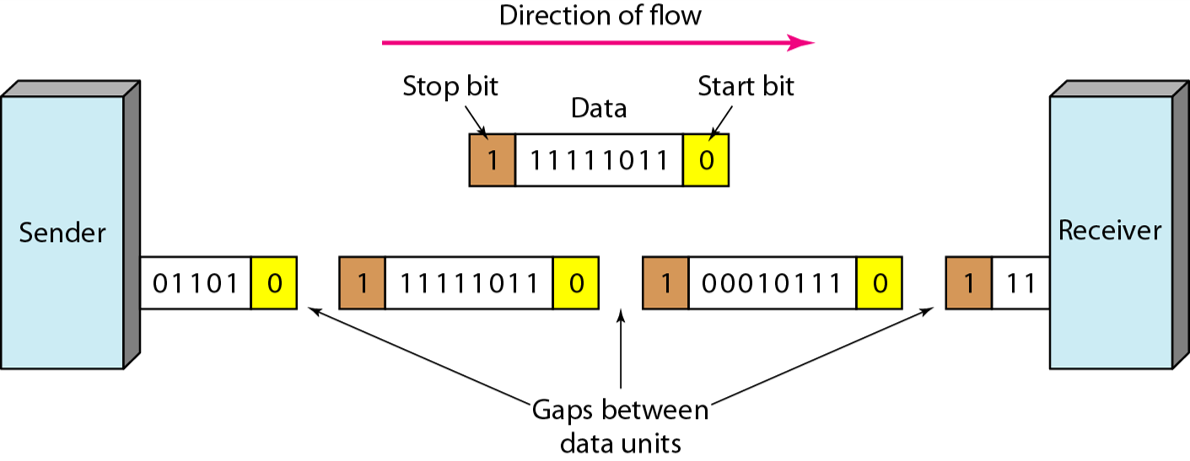
\includegraphics[width=0.9\columnwidth]{bab4/Picture34.png}
  \caption{Asynchronous transmission}
  \label{fig4:34}
\end{figure}


\subsection*{Synchronous Transmission}
In synchronous transmission, the bit stream is combined into longer "frames," which may contain multiple bytes. Each byte, however, is introduced onto the transmission link without a gap between it and the next one. It is left to the receiver to separate the bit stream into bytes for decoding purposes. In other words, data are transmitted as an unbroken string of 1s and Os, and the receiver separates that string into the bytes, or characters, it needs to reconstruct the information. In synchronous transmission, we send bits one after another without start or stop bits or gaps. It is the responsibility of the receiver to group the bits.

Figure 4.35 gives a schematic illustration of synchronous transmission. We have drawn in the divisions between bytes. In reality, those divisions do not exist; the sender puts its data onto the line as one long string. If the sender wishes to send data in separate bursts, the gaps between bursts must be filled with a special sequence of Os and Is that means idle. The receiver counts the bits as they arrive and groups them in 8-bit units.

\begin{figure}
  \centering
  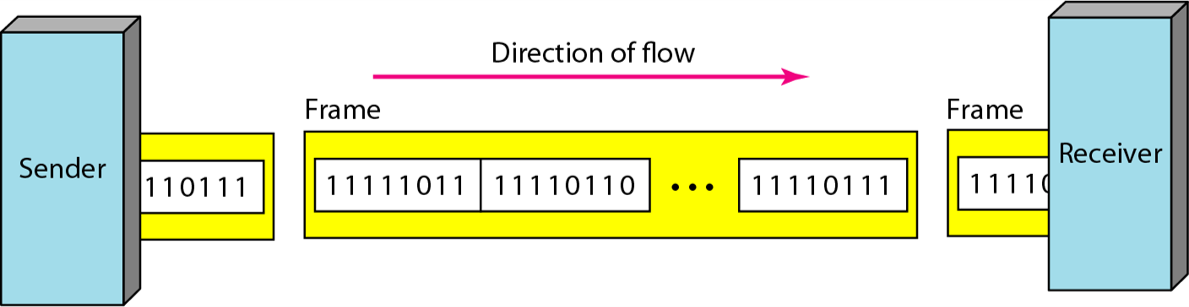
\includegraphics[width=0.9\columnwidth]{bab4/Picture35.png}
  \caption{Synchronous transmission}
  \label{fig4:35}
\end{figure}

Without gaps and start and stop bits, there is no built-in mechanism to help the receiving device adjust its bit synchronization midstream. Timing becomes very important, therefore, because the accuracy of the received information is completely dependent on the ability ofthe receiving device to keep an accurate count of the bits as they come in. The advantage of synchronous transmission is speed. With no extra bits or gaps to introduce at the sending end and remove at the receiving end, and, by extension, with fewer bits to move across the link, synchronous transmission is faster than asynchronous transmission. For this reason, it is more useful for high-speed applications such as the transmission of data from one computer to another. Byte synchronization is accomplished in the data link layer. We need to emphasize one point here. Although there is no gap between characters in synchronous serial transmission, there may be uneven gaps between frames.


\subsection*{Isochronous}
In real-time audio and video, in which uneven delays between frames are not acceptable, synchronous transmission fails. For example, TV images are broadcast at the rate of 30 images per second; they must be viewed at the same rate. If each image is sent by using one or more frames, there should be no delays between frames. For this type of application, synchronization between characters is not enough; the entire stream of bits must be synchronized. The isochronous transmission guarantees that the data arrive at a fixed rate.

\section{Ringkasan}
\begin{itemize}
  \item[$\odot$] Digital-to-digital conversion involves three techniques: line coding, block coding, and scrambling.
  \item[$\odot$] Line coding is the process of converting digital data to a digital signal.
  \item[$\odot$] We can roughly divide line coding schemes into five broad categories: unipolar, polar, bipolar, multilevel, and multitransition
  \item[$\odot$] Block coding provides redundancy to ensure synchronization and inherent error detection. Block coding is normally referred to as mB/nB coding; it replaces each m-bit group with an n-bit group
\end{itemize}

\section{Latihan}

\subsection*{Pertanyaan ulasan}

\begin{enumerate}
  \item Describe the goals of multiplexing.
  \item List three main multiplexing techniques mentioned in this chapter. 
  \item Distinguish between a link and a channel in multiplexing. 
  \item Which of the three multiplexing techniques is (are) used to combine analog signals? Which ofthe three multiplexing techniques is (are) used to combine digital signals? 
  \item Define the analog hierarchy used by telephone companies and list different levels ofthe hierarchy. 
  \item Define the digital hierarchy used by telephone companies and list different levels of the hierarchy. 
  \item Which of the three multiplexing techniques is common for fiber optic links? Explain the reason. 
  \item Distinguish between multilevel TDM, multiple slot TDM, and pulse-stuffed TDM. 
  \item Distinguish between synchronous and statistical TDM. 
  \item Define spread spectrum and its goal. List the two spread spectrum techniques discussed in this chapter. 
  \item Define FHSS and explain how it achieves bandwidth spreading. 
  \item Define DSSS and explain how it achieves bandwidth spreading.
\end{enumerate}

\subsection*{Latihan}
\begin{enumerate}[resume]
  \item Assume that a voice channel occupies a bandwidth of 4 kHz. We need to multiplex 10 voice channels with guard bands of 500 Hz using FDM. Calculate the required bandwidth.
  \item We need to transmit 100 digitized voice channels using a pass-band channel of 20 KHz. What should be the ratio of bits/Hz if we use no guard band?
  \item In the analog hierarchy of Figure 6.9, find the overhead (extra bandwidth for guard band or control) in each hierarchy level (group, supergroup, master group, and jumbo group)
  \item We need to use synchronous TDM and combine 20 digital sources, each of 100 Kbps. Each output slot carries 1 bit from each digital source, but one extra bit is added to each frame for synchronization. Answer the following questions
  \item Repeat Exercise 16 if each output slot carries 2 bits from each source
  \item We have 14 sources, each creating 500 8-bit characters per second. Since only some of these sources are active at any moment, we use statistical TDM to combine these sources using character interleaving. Each frame carries 6 slots at a time, but we need to add four-bit addresses to each slot. Answer the following questions:
  \item Ten sources, six with a bit rate of 200 kbps and four with a bit rate of 400 kbps are to be combined using multilevel TDM with no synchronizing bits. Answer the following questions about the final stage of the multiplexing
  \item Four channels, two with a bit rate of 200 kbps and two with a bit rate of 150 kbps, are to be multiplexed using multiple slot TDM with no synchronization bits. Answer the following questions:
  \item Two channels, one with a bit rate of 190 kbps and another with a bit rate of 180 kbps, are to be multiplexed using pulse stuffing TDM with no synchronization bits. Answer the following questions:
  \item Answer the following questions about a T-1 line:
  \item Show the contents of the five output frames for a synchronous TDM multiplexer that combines four sources sending the following characters. Note that the characters are sent in the same order that they are typed. The third source is silent
  \item Figure 6.34 shows a multiplexer in a synchronous TDM system. Each output slot is only 10 bits long (3 bits taken from each input plus 1 framing bit). What is the output stream? The bits arrive at the multiplexer as shown by the arrows
  \item Figure 6.35 shows a demultiplexer in a synchronous TDM. If the input slot is 16 bits long (no framing bits), what is the bit stream in each output? The bits arrive at the demultiplexer as shown by the arrows
  \item Answer the following questions about the digital hierarchy in Figure 6.23
  \item What is the minimum number of bits in a PN sequence if we use FHSS with a channel bandwidth of B =4 KHz and Bss =100 KHz?
  \item An FHSS system uses a 4-bit PN sequence. If the bit rate of the PN is 64 bits per second, answer the following questions:
  \item A pseudorandom number generator uses the following formula to create a random series:
  \item We have a digital medium with a data rate of 10 Mbps. How many 64-kbps voice channels can be carried by this medium if we use DSSS with the Barker sequence?
\end{enumerate}
